\documentclass{article}
\usepackage{mathtools}
%\usepackage{natbib}
\usepackage[numbers]{natbib}
\usepackage[utf8]{inputenc}
\usepackage{graphicx}
\usepackage{url}
\usepackage{array,multirow,makecell}
\usepackage[T1]{fontenc}
\usepackage{setspace}
\usepackage{accents}
\usepackage{color}
\usepackage{enumitem}
\usepackage[11pt]{extsizes}
\usepackage{layout}
\usepackage[top=3cm, bottom=3cm, left=2cm, right=2cm]{geometry}
\usepackage[colorlinks=true,linkcolor=blue]{hyperref}
\usepackage{systeme}
\usepackage[standard]{ntheorem}
\usepackage{pgfplots}
\pgfplotsset{width=8cm,compat=1.9}
\usepackage{comment}
\usepackage{tabularray}
\usepackage{pgfplotstable}
\usepackage{xspace}
\usepgfplotslibrary{statistics}
\usepackage{algorithm,algpseudocode}
\usepackage{authblk}
\usepackage{bm}
\usepackage{appendix}

\usepackage{subcaption}
\usepackage{tikz}
\usepackage{adjustbox}


\newcommand{\q}[1]{``#1''}
\DeclareMathOperator*{\esssup}{ess\,sup}
\DeclareMathOperator{\diag}{diag}
\renewcommand\Authfont{\fontsize{12}{14.4}\selectfont}

\DeclareGraphicsExtensions{.pdf,.png}
\renewcommand{\q}[1]{``#1''}

\pagestyle{plain}

\title{Swing Contract Pricing: A Parametric Approach with Adjoint Automatic Differentiation and Neural Networks}

\author[1]{Vincent Lemaire}
\author[1]{Gilles Pagès}
\author[1,2]{Christian Yeo}
\affil[1]{\footnotesize Sorbonne Université, Laboratoire de Probabilités, Statistique et Modélisation, UMR 8001, case 158, 4, pl. Jussieu,
F-75252 Paris Cedex 5, France}
\affil[2]{\footnotesize Engie Global Markets, 1 place Samuel Champlain, 92400 Courbevoie, France}

\date{}


\numberwithin{equation}{section}
\begin{document}


\maketitle

\begin{abstract}
    We propose two parametric approaches to price swing contracts with firm constraints. Our objective is to create approximations for the optimal control, which represents the amounts of energy purchased throughout the contract. The first approach involves explicitly defining a parametric function to model the optimal control, and the parameters using stochastic gradient descent-based algorithms. The second approach builds on the first one, replacing the parameters with neural networks. Our numerical experiments demonstrate that by using Langevin-based algorithms, both parameterizations provide, in a short computation time, better prices compared to state-of-the-art methods (like the one given by Longstaff and Schwartz).
\end{abstract}

\textit{\textbf{Keywords} - Swing contracts, stochastic control, stochastic approximation, neural network, Langevin dynamics, greeks.}


\vspace{0.6cm}


\section*{Introduction}
\indent

With the energy market becoming increasingly deregulated, various derivative products have emerged, offering flexibility in delivery dates and purchased energy amounts. \q{Swing} contracts, also known as \q{Take-or-Pay} contracts (see \cite{Thompson1995ValuationOP} for more details), are among the most widely traded contracts in gas and power markets. These contracts allow their holders to purchase amounts of energy on fixed exercise dates, subject to certain constraints. There exist two types of constraints. In the firm constraints setting, the contract holder is not allowed to violate the constraints. Beside this case, there exists an alternative setting where the holder can violate them but will face a penalty proportional to the default. Our paper focuses on the valuation of swing contracts in the firm constraints case.


The valuation of swing contracts is a more challenging task than that of classic American-style contracts \cite{Broadie2004ASM, Jaillet1990VariationalIA, Longstaff2001ValuingAO, Rogers2002MonteCV}, mainly due to the presence of constraints related to time and volume. From a probabilistic standpoint, the valuation of swing contracts is related to a Stochastic Optimal Control (\textit{SOC}) problem. Here, the control represents the vector of amounts of energy that can be purchased at each exercise date. To solve this SOC problem, two primary groups of methods have been developed.


The first group concerns methods that are based on the so called \q{Backward Dynamic Programming Principle} (BDPP). In this group, the price of the swing contract can be written as a solution of a dynamic programming equation (see \cite{Bardou2007WhenAS, Bardou2009OptimalQF, BarreraEsteve2006NumericalMF,Jaillet2004ValuationOC, LariLavassani2002ADV,Thompson1995ValuationOP}). More precisely, at each exercise date, given the underlying price and the cumulative consumption, the contract value is given by the maximum over the possible consumptions of the immediate cash flow plus the (conditional) expected value of future cash flows. The latter amount (which is in fact a conditional expectation) is often called the \q{continuation value} and its evaluation is the main difficulty when consider BDPP-based approaches. The mostly used method for computing the continuation value is the Longstaff and Schwartz one (see \cite{Longstaff2001ValuingAO}); where the continuation value is approximated as an orthogonal projection over a subspace spanned by a finite number of squared integrable random variables (see \cite{BarreraEsteve2006NumericalMF, Longstaff2001ValuingAO}). Another method is based on the so called optimal quantization (see \cite{Pags2004OptimalQM}) where the underlying (continuous) random variable is approximated by its discrete version which in turns is defined by a \q{projection} on nearest neighbors or Voronoï cells (see \cite{Bardou2009OptimalQF}). Thus the continuation value reduces to a conditional expectation of a discrete random variable. One of the major problems with BDPP's approaches is the following. To compute the value of the contract at each exercise date, the maximum is taken over a geometric interval. In practice the latter interval needs to be discretized leading to a precision/complexity tradeoff. Indeed, achieving a high level of accuracy in pricing the contract requires a finer discretization of the geometric interval, which in turn increases computation time. Additionally, the Longstaff-Schwartz method faces a storage challenge, as regression coefficients for each simulation and admissible cumulative consumption must be stored at each exercise date to compute the continuation value. This often leads to a memory overflow when a large number of simulations is required to obtain a price with a tight confidence interval. Meanwhile, the optimal quantization method suffers from the \q{curse of dimensionality} because it is well known that the rate of convergence of this method is of order $\mathcal{O}(N^{-\frac{1}{d}})$ (where $N$ is the number of simulations and $d$ is the problem dimension).


An alternative approach to BDPP-based methods is to consider the valuation of swing contracts as a global optimization problem. As mentioned, the valuation of swing contract is equivalent to solve a SOC problem where the objective is to find a vector of purchase amounts that maximizes the expected value of cumulative cash flows up to the expiry of the contract. This leads to a stochastic optimization problem where the control is generally substituted by a parametric function, and optimal parameters are identified using Stochastic Gradient Descent (SGD) algorithms. The use of parametric functions to approximate the optimal control reduces the control problem to a parametric optimization problem. However, the success of such approaches is contingent upon finding a suitable parametric function, which often requires a solid understanding and intuition of the optimal control's behavior. Note that, solving SOC problem with SGD based algorithms have been considered in \cite{GobetMunos} for general SOC problems and in \cite{BarreraEsteve2006NumericalMF} for the swing contracts case. To the best of our knowledge, there has been limited exploration of such approaches in the literature to price swing options. Thus, in this paper, we propose two parametric methods for global optimization and compare them with the Longstaff-Schwartz method. We optimize both parameterizations using two algorithms: Adaptive Moment Estimation (Adam) and (Preconditioned) Stochastic Gradient Langevin (PSGLD). While Adam is widely used in stochastic approximation, PSGLD has demonstrated effectiveness in recent studies for Bayesian learning. Our results show that using Langevin-type algorithms can accelerate the training of our parameterizations and leads to better prices compared to the state-of-the-art methods.


Our paper is organized as follows. Section \ref{sec1}. We describe swing contracts and recall the pricing framework. Section \ref{sec2}. We present our contribution by proposing two numerical methods for the pricing of swing contracts. Section \ref{training_part}. We present generalities about stochastic approximation and study two optimization algorithms to optimize our numerical solutions. Finally in section \ref{sec5} we present some additional results about the effectiveness of our methods.



\section{On swing contracts}
\label{sec1}

\indent

In this section, we will provide an overview of swing contracts and explain how to build the swing volume grid defining the space of volume constraints. In a firm constraints setting, this space is a critical component to price swing contracts, and this will discussed towards the end of this section.


\subsection{Description}

\indent

Swing option is a commonly encountered derivative on energy (gas and power) markets which allows its holder to buy amounts of energy $q_{k}$ at times $t_k$, $k = 0, ...,n-1$ (called exercise dates) until the contract maturity $t_n = T$. At each exercise date $t_k$, the purchase price (or strike price of the contract) is denoted $K_k$ and can be constant (i.e $K_k = K, k = 0,...,n-1$) or indexed on a formula. In this paper, we focus on the fixed strike price case but the case of indexed strike can be treated likewise. In this latter case the strike at a time $t_k$ is often calculated as the average of the underlying prices over a period which is already completed. Therefore the indexed strike price case only adds a computational complexity rather than a theoretical one.


One important feature on swing option are volume constraints. Swing option gives its holder a flexibility on the amount of energy he is allowed to purchase and this flexibility is subject to some (firm) constraints

\begin{itemize}
    \item \textbf{Local constraints}: at each exercise date $t_k$, the holder of the swing contract is allowed to buy at least $q_{\min}$ and at most $q_{\max}$ i.e,
    
    \begin{equation}
    \label{loc_const}
    q_{\min} \le q_{k} \le q_{\max}, \hspace{0.5cm} 0 \le k \le n-1.
    \end{equation}
    
    
    \item \textbf{Global constraints}: the cumulative consumption up to the maturity of the contract must be not lower than $Q_{\min}$ and not greater than $Q_{\max}$ i.e,
    
    \begin{equation}
    \label{glob_const}
    Q_{n} = \sum_{k = 0}^{n-1} q_{k} \in [Q_{\min}, Q_{\max}], \hspace{0.4cm} \text{with} \hspace{0.2cm} Q_0 = 0 \hspace{0.1cm} \text{and} \hspace{0.1cm} 0 \le Q_{\min} \le Q_{\max} \le +\infty.
    \end{equation}

\end{itemize}


Note that in this paper we only consider the \textbf{firm constraints} case which means that the holder of the contract is not allowed to violate the constraints. This case is often released in the literature by adding a penalty term whenever the global constraints are violated (see \cite{Bardou2009OptimalQF, BarreraEsteve2006NumericalMF}). In penalty setting, the existence of an optimal Markov consumption had been proved in \cite{BarreraEsteve2006NumericalMF} using a smooth penalty function. A similar result has been established in \cite{Bardou2007WhenAS} for the firm constraints case.



Now let us focus on the firm constraints case in which one of the main components is the physical space. That is the area of possible actions taking into account the volume constraints.


\subsection{Physical space}
\label{physical_space}

\indent

At each exercise date, through the firm constraints, the achievable cumulative volumes are delimited by boundaries represented by the functions $t_k \mapsto Q^{down}(t_k)$ and $t_k \mapsto Q^{up}(t_k)$

\vspace{0.1cm}

\begin{equation}
\left\{
    \begin{array}{ll}
        Q^{down}(t_0) = 0\\
        \displaystyle Q^{down}(t_k) = \max\big(0, Q_{\min} - (n-k) \cdot q_{\max} \big) \hspace{0.3cm} \text{,} \hspace{0.1cm} k \in \{1,...,n-1\} \\
        Q^{down}(t_n) = Q_{\min}
    \end{array}
\right.
\end{equation}

\vspace{0.1cm}

\begin{equation}
\left\{
    \begin{array}{ll}
        Q^{up}(t_0) = 0\\
        \displaystyle Q^{up}(t_k) = \min\big(k \cdot q_{\max}, Q_{\max}\big) \hspace{0.3cm} \text{,} \hspace{0.1cm} k  \in \{1,...,n-1\}\\
        Q^{up}(t_n) = Q_{\max}
    \end{array}
\right.
\end{equation}

\vspace{0.2cm}

\noindent
where $Q^{down}(t_k)$ and $Q^{up}(t_k)$ denote respectively the lower and the upper bound of the cumulative consumption at time $t_k$. These boundaries lead to the physical space of the swing contract, as drawn in Figure \ref{physical space swing} and represents at each exercise date, the range of attainable cumulative consumptions.


\begin{figure}[!ht]
    \center
    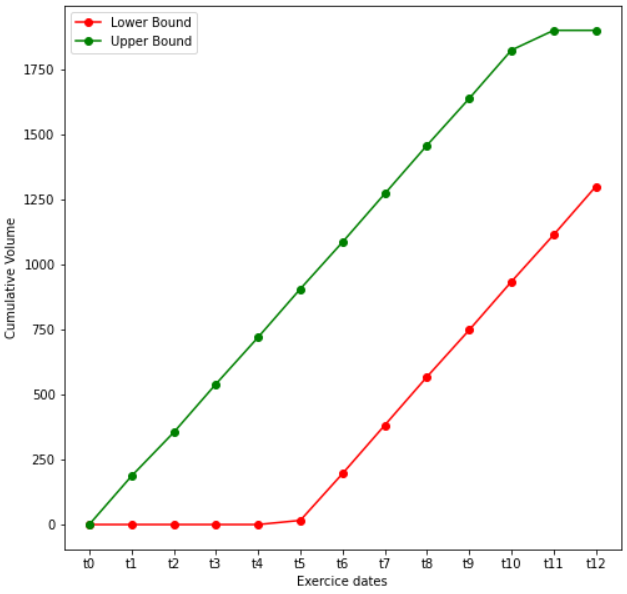
\includegraphics[scale=0.3]{Images/swing_grid_eg.PNG}
    \caption{Illustration of swing physical space with $q_{\min} = 0, q_{\max} = 180, Q_{\min} = 1300, Q_{\max} = 1900$ and 12 exercise dates.}
    \label{physical space swing}
\end{figure}

\noindent
In Figure \ref{physical space swing} we assumed that $q_{\min} = 0$. This assumption can be made without loss of generality because, as shown in \cite{Bardou2009OptimalQF}, the general case can always be reduced to the case where $q_{\min} = 0$ and $q_{\max} = 1$ (see appendix \ref{swing decompo} for the proof). Besides, if at an exercise date $t_k$ we have bought the amounts $q_{0},...,q_{k-1}$ leading to a cumulative consumption $\displaystyle Q_k = \sum_{i = 0}^{k -1} q_i$, then due to local constraints and the cumulative consumption borders, the actual range of attainable cumulative consumption at time $t_{k+1}$ is the following

\begin{equation}
    Q_k + q_k \in \Big[\underbrace{\max(Q^{down}(t_{k+1}), Q_{k} + q_{\min})}_{:= L_{{k+1}}(Q_k)}, \hspace{0.2cm}  \underbrace{\min(Q^{up}({k+1}), Q_{k} + q_{\max})}_{:= U_{{k+1}}(Q_k)}\Big].
    \label{range_cum_vol}
\end{equation}

\noindent
That is, starting with a cumulative consumption $Q_{k}$, at time $t_k$, the range of admissible volume is

\begin{equation}
    q_k \in \Big[\underbrace{L_{{k+1}}(Q_k) - Q_k}_{:= A_k^{-}(Q_k)}, \hspace{0.2cm}  \underbrace{U_{{k+1}}(Q_k) - Q_k}_{:= A_k^{+}(Q_k)}\Big].
    \label{intervalle_control}
\end{equation}


With theses basic blocks, we can now set the theoretical framework for the pricing of swing contracts.


\subsection{Pricing and sensitivity calculus}
\label{pricing}

\indent

Let $\left(\Omega, \mathcal{F}, \{ \mathcal{F}_t \}, \mathbb{P} \right)$ be a filtered probability space. The price at time $t$ of the forward contract delivered at the maturity $T$ is denoted by $F_{t, T}$. In this paper (as in \cite{Bardou2009OptimalQF, BarreraEsteve2006NumericalMF}) we consider contract on the spot price ($S_t = F_{t,t}$) even if in practice the spot is not a tradable instrument on market. Instead, the most encountered gas contract is the day-ahead forward contract whose price is  $F_{t, t+1}$. But this case can be treated in the same way.

The decision process $(q_{k})_{0 \le k \le n-1}$ is defined on the same probability space and is supposed $\mathcal{F}_{t_k}^S$- adapted. At each exercise date $t_k$, by buying a certain volume $q_k$, the holder of the contract makes a profit (or loss)

\begin{equation}
\psi_k\left(q_{k}, S_{t_k} \right) := q_{k} \cdot\left(S_{t_k} - K\right).
\end{equation}

Let $Q \in \mathbb{R}_{+}$. Given a cumulative consumption $Q$, an admissible strategy at time $t_k$ is a vector $(q_k, \ldots, q_{n-1})$ lying within the following set

\begin{equation*}
\mathcal{A}_{k, Q}^{Q_{\min}, Q_{\max}} = \left\{(q_{\ell})_{k \le \ell \le n-1}, \hspace{0.1cm} q_{\ell} : (\Omega, \mathcal{F}_{t_{\ell}}^S, \mathbb{P}) \mapsto [q_{\min}, q_{\max}], \hspace{0.1cm} \sum_{\ell = k}^{n-1} q_{\ell} \in \big[(Q_{\min}-Q)_{+}, Q_{\max}-Q \big] \right\}.
\end{equation*}

\noindent
Note that using equation \eqref{intervalle_control}, the preceding set reads,

\begin{equation}
\label{actual_set_adm_const_case}
\mathcal{A}_{k, Q}^{Q_{\min}, Q_{\max}} = \left\{(q_{\ell})_{k \le \ell \le n-1}, \hspace{0.1cm} q_{\ell} : (\Omega, \mathcal{F}_{t_{\ell}}^S, \mathbb{P}) \mapsto \big[A_\ell^{-}(Q_\ell), A_\ell^{+}(Q_\ell) \big], \hspace{0.1cm} \text{where} \hspace{0.1cm} Q_\ell = Q + \sum_{i = k}^{\ell - 1} q_i \right\}.
\end{equation}

\noindent
with the convention $\displaystyle \sum_{i = k}^{k - 1} q_i = 0$. Then for every non negative $\mathcal{F}_{t_{k-1}}^S-$ measurable random variable $Q$, the price of the swing option at time $t_k$ starting from a cumulative consumption $Q$ is given by

\begin{equation}
    P_k\left(S_{t_k}, Q \right) = \esssup_{(q_{\ell})_{k \le \ell \le n-1} \in \mathcal{A}_{k, Q}^{Q_{\min}, Q_{\max}}} \hspace{0.1cm} \mathbb{E}\left(\sum_{\ell=k}^{n-1} e^{-r_\ell(t_{\ell} - t_k)} \psi_\ell\left(q_{\ell}, S_{t_{\ell}} \right) \rvert \mathcal{F}_{t_k}^S \right),
    \label{pricing_swing_formula}
\end{equation}


\noindent
where the expectation is taken under the risk-neutral probability and $r_{\ell}$ are interest rates over the period $[t_0, t_{n-1}]$ that we will assume to be zero throughout this paper. Then the price of the swing contract is given by ($S_{t_0}$ is assumed to be deterministic)

\begin{equation}
    P_0 := P_0\big(S_{t_0}, 0\big) = \underset{(q_\ell)_{0 \le \ell \le n-1} \in \mathcal{A}_{0, 0}^{Q_{\min}, Q_{\max}}}{\sup} \hspace{0.1cm}  \mathcal{J}\big(q_0, \ldots, q_{n-1}\big).
    \label{swing_init_price}
\end{equation}


\noindent
where, given an admissible strategy $(q_0, \ldots, q_{n-1})$, the reward function $\mathcal{J}$ is defined as the expected value of cumulative future cash flows up to the expiry

\begin{equation}
\mathcal{J}\big(q_0, \ldots, q_{n-1}\big) := \mathbb{E}\left(\sum_{\ell=0}^{n-1} \psi_{\ell}\big(q_{\ell}, S_{t_{\ell}} \big)\right).
\end{equation}

The latter problem appears to be a constrained stochastic control problem in which the aim is to find an admissible strategy that maximizes the reward function $\mathcal{J}$. As mentioned in the introduction, there exists in the literature two groups of pricing methods to solve this optimization problem. The first group of methods is based on the \q{backward dynamic programming principle} and the second on a global optimization approach. In this paper, we propose two numerical solutions to solve problem \eqref{swing_init_price} based on this latter group. 


It is important to note the \q{bang-bang} feature, which implies that under certain conditions, at each exercise date, the optimal consumption is given by one of two values: $A_k^-$ or $A_k^+$ (defined in equation \eqref{intervalle_control}). This feature has been proven for the case of firm constraints and when global constraints are whole numbers by Pagès et al. \cite{Bardou2007WhenAS}. For the penalty case, a proof can be found in Gobet et al. \cite{BarreraEsteve2006NumericalMF}. The \q{bang-bang} feature is particularly valuable since it allows to significantly reduce the computation time it.

In this paper and unless otherwise stated, we use a one-factor model as in \cite{BarreraEsteve2006NumericalMF, Jaillet2004ValuationOC}. That is,

\begin{equation}
	\frac{dF_{t, T}}{F_{t_, T}} = \sigma e^{-\alpha (T-t)}dW_t, \hspace{0.4cm}  t \le T
	\label{hjm_model}
\end{equation}

\noindent
where $W$ is a standard Brownian motion. As mentioned before we deal with the spot price whose price is given by a straightforward application of Itô formula

\begin{equation}
\label{spot_model}
S_t = F_{0,t} \cdot \exp\big(\sigma X_t - \frac{1}{2}\lambda_t^2\big), \hspace{0.3cm} X_t = \int_{0}^{t} e^{-\alpha (t-s)}\, \mathrm{d}W_s \hspace{0.3cm} \text{and} \hspace{0.3cm} \lambda_t^2 = \frac{\sigma^2}{2\alpha}\big(1-e^{-2\alpha t}\big).
\end{equation}

\noindent
Along with this model, we will use two settings (presented below). In each case we set $\alpha = 4, \sigma = 0.7$.

\vspace{0.3cm}

\textbf{Case 1}

\begin{center}
31 exercise dates \hspace{0.4cm} $q_{\min} = 0 \hspace{0.4cm} q_{\max} = 6 \hspace{0.4cm} Q_{\min} = 140 \hspace{0.4cm} Q_{\max} = 200$. 
\end{center}


\textbf{Case 2} (as in \cite{Bardou2009OptimalQF, BarreraEsteve2006NumericalMF})

\begin{center}
365 exercise dates \hspace{0.4cm} $q_{\min} = 0 \hspace{0.4cm} q_{\max} = 6 \hspace{0.4cm} Q_{\min} = 1300 \hspace{0.4cm} Q_{\max} = 1900$.
\end{center}

The computer that has been used has the following characteristics: \textit{Processor: Intel(R) Core(TM) i7-1185G7 @ 3.00GHz   3.00 GHz, 32Go of RAM, Microsoft Windows 10 Enterprise}. Deep learning part had been implemented using PyTorch toolbox. The GPU device used is: Nvidia A100-PCIE 40GB.

\vspace{0.2cm}

It is worth noting that for practitioners, the prices of derivatives are closely linked to their sensitivities with respect to market data. These sensitivities are essential for hedging purposes, as they indicate how the price of a derivative product changes with the market. Computation of sensitivities involves calculating derivatives, and in our case, we need to differentiate a price with respect to some parameters, where the price is a solution to the stochastic control problem in equation \eqref{swing_init_price}. To achieve this, we rely on the so called \q{envelope theorem.}

\vspace{0.2cm}

Let $f(x,\alpha)$ and  $g_{j}(x,\alpha),j=1,2,\ldots ,m$ be real-valued continuously differentiable functions on $\mathbb{R}^{n+\ell}$ , where $x\in \mathbb {R} ^{n}$ are some variables and $\alpha \in \mathbb {R}^{\ell}$ are parameters, and consider the constrained optimization problem

$$
\left\{
    \begin{array}{ll}
        \underset{x}{\max} \hspace{0.1cm} f(x, \alpha)\\
        \text{subject to} \hspace{0.2cm} g_{j}(x,\alpha) \ge 0, \hspace{0.4cm} 1 \le j \le m
    \end{array}
\right.
$$

\noindent
We introduce the Lagrangian function,

$$\mathcal{L}\left(x, \lambda, \alpha \right) = f(x, \alpha) + \langle\lambda, g(x, \alpha) \rangle $$

\noindent
where $\lambda \in \mathbb{R}^{m}$ is the Lagrange multipliers, $\langle \cdot,\cdot \rangle$ is the Euclidean inner-product and $g = (g_1, \ldots, g_m)^\top$. Then we define the value function $V(\alpha) = f(x^{*}(\alpha), \alpha)$ where $x^{*}(\alpha)$ is a solution that maximizes the function $f(\cdot, \alpha)$. The following theorem gives the derivative of the value function $V$ in case it is differentiable.

\begin{theorem}[Envelope theorem]
\label{env_thm}
Assume that $V$ and $\mathcal {L}$ are continuously differentiable. Then,

$$\frac{\partial V(\alpha)}{\partial \alpha_k} = \frac{\partial \mathcal{L}\left(x^{*}(\alpha), \lambda^{*}(\alpha), \alpha  \right)}{\partial \alpha_k} \hspace{0.7cm} k=1,\ldots,\ell$$
\noindent
where $\frac{\partial \mathcal{L}}{\partial \alpha_k} = \frac{\partial f}{\partial \alpha_k} + \langle\lambda, \frac{\partial g}{\partial \alpha_k}\rangle.$

\end{theorem}

The envelope theorem states that, under some regularity conditions, in a SOC problem, for example our problem \eqref{swing_init_price}, the derivative of the optimal objective function $\mathcal{J}$ is given by differentiating the cash flows along with the optimal control. In our model \eqref{hjm_model}, we deduce the following proposition which is a corollary application of Theorem \ref{env_thm}.

\begin{Proposition}

Let $\left(q_{k}^{*} \right)_{0 \le k \le n-1}$ be a solution of the problem \eqref{swing_init_price}. Assume that the function

$$\left(F_{0, t_k} \right)_{0 \le k \le n-1} \mapsto \mathbb{E}\left(\sum_{k = 0}^{n-1} q_{k}^{*} \cdot \left( F_{0, t_k} \cdot e^{\sigma X_{t_k} - \frac{1}{2}\Lambda_{t_k}} - K \right) \right)$$

\noindent
is continuously differentiable. Let $P_0$ be the price of the swing contract \eqref{swing_init_price}. Note that $P_0$ is a function of $\big(S_{t_k})_{0 \le k \le n-1}$ which in turns depends on $\big(F_{0,t_k})_{0 \le k \le n-1}$ in the model \eqref{hjm_model}. Then for all $k = 0,\ldots, n-1$, the delta (sensitivity of swing price with respect to the initial forward price) is given by

$$\frac{\partial P_0}{\partial F_{0, t_k}} = \mathbb{E}\left(q_{k}^{*} \cdot e^{\sigma X_{t_k} - \frac{1}{2}\Lambda_{t_k} } \right).$$


\end{Proposition}

\begin{proof}
We define the following functions:


$$f\left((q_{k})_{0 \le k \le n-1}, (F_{0, t_k})_{0 \le k \le n-1} \right) := \mathbb{E}\left(\sum_{k = 0}^{n-1} q_{k} \cdot \left( F_{0, t_k} \cdot e^{\sigma X_{t_k} - \frac{1}{2}\Lambda_{t_k}} - K \right) \right)$$


$$g_1\left((q_{k})_{0 \le k \le n-1}, (F_{0, t_k})_{0 \le k \le n-1}\right) := \sum_{k=0}^{n-1} q_{k} - Q_{\min}$$

$$g_2\left((q_{k})_{0 \le k \le n-1}, (F_{0, t_k})_{0 \le k \le n-1}\right) := Q_{\max}- \sum_{k=0}^{n-1} q_{k} $$

\noindent
and for all $k = 0, \ldots, n-1$:

$$g_{2k+3}\left((q_{k})_{0 \le k \le n-1}, (F_{0, t_k})_{0 \le k \le n-1}\right) := q_{k} - q_{\min}$$

$$g_{2k+4}\left((q_{k})_{0 \le k \le n-1}, (F_{0, t_k})_{0 \le k \le n-1}\right) := q_{\max} - q_{k}$$

\noindent
Then it suffices to prove that functions $f, g_1, g_2, \ldots, g_{2n+2}$ are continuously differentiable in order to use the envelope theorem. This holds for functions $g_1, g_2, \ldots, g_{2n+2}$. It remains to prove it for function $f$. The latter reduces to show that function $f$ is continuously differentiable in each of its components. For any $k = 0, \ldots, n-1$, the random variable $q_{k} \cdot \big(F_{0, t_k} \cdot e^{\sigma X_{t_k} - \frac{1}{2}\Lambda_{t_k}} - K \big)$ is integrable since

$$\Big|q_{k} \cdot \big(F_{0, t_k} \cdot e^{\sigma X_{t_k} - \frac{1}{2}\Lambda_{t_k}} - K \big)\Big| \le q_{\max} \cdot \big( F_{0, t_k} \cdot e^{\sigma X_{t_k} - \frac{1}{2}\Lambda_{t_k}} + K \big) \in \mathbb{L}_\mathbb{R}^1(\mathbb{P}).$$

\noindent
Moreover, the function $F_{0, t_k} \mapsto q_{k} \cdot\big(F_{0, t_k} \cdot e^{\sigma X_{t_k} - \frac{1}{2}\Lambda_{t_k}} - K \big)$ is differentiable and its derivative does not depends on $F_{0, t_k}$. Furthermore,

\begin{align*}
\Big|\frac{\partial}{\partial F_{0, t_k}} \Big(q_{k} \cdot \big(F_{0, t_k} \cdot e^{\sigma X_{t_k} - \frac{1}{2}\Lambda_{t_k}} - K \big) \Big)\Big| = \big|q_{k} \cdot e^{\sigma X_{t_k} - \frac{1}{2}\Lambda_{t_k}} \Big| \le q_{\max} \cdot e^{\sigma X_{t_k}} \in \mathbb{L}_\mathbb{R}^1(\mathbb{P}).
\end{align*}

\noindent
Then thanks to Lebesgue theorem to interchange derivation and integral, the function $f$ is continuously differentiable in all $F_{0, t_k}$. Likewise one may also show that for all $k = 0, \ldots, n-1$ the function $f$ is continuously differentiable in $q_{k}$, and one may use the envelope theorem. For any $k=0,\ldots,n-1$ we introduce the Lagrangian of the problem \eqref{swing_init_price}

\begin{align*}
	\mathcal{L}\left((q_{k})_{0 \le k \le n-1},\lambda, \left(F_{0, t_k}\right)_{0 \le k \le n-1} \right) &= \mathbb{E}\left(\sum_{k = 0}^{n-1} q_{k} \cdot \left( F_{0, t_k} \cdot e^{\sigma X_{t_k} - \frac{1}{2}\Lambda_{t_k}} - K \right) \right) +\\
	& \langle \lambda, g\big((q_{k})_{0 \le k \le n-1}, (F_{0, t_k})_{0 \le k \le n-1} \big) \rangle,
\end{align*}

\noindent
where $g = \left(g_1, \ldots, g_{2n+2}\right)^\top$ and $\lambda \in \mathbb{R}^{2n+2}$. Then it follows from envelope theorem that for any $k = 0, \ldots, n-1$:

\begin{align*}
\frac{\partial P_0}{\partial F_{0, t_k}} = \mathbb{E}\left(\sum_{k = 0}^{n-1} q_{k}^{*} \cdot \frac{\partial}{\partial F_{0, t_k}} \left( F_{0, t_k} \cdot e^{\sigma X_{t_k} - \frac{1}{2}\Lambda_{t_k}} - K \right) \right) = \mathbb{E}\left(\sum_{k = 0}^{n-1} q_{k}^{*} \cdot e^{\sigma X_{t_k} - \frac{1}{2}\Lambda_{t_k}} \right).
\end{align*}

\noindent
This completes the proof. 

\end{proof}


We have outlined the theoretical framework for pricing swing contracts and computing their associated sensitivities. To obtain practical numerical solutions, we introduce parametric methods in this paper. Specifically, we replace the optimal control variable $q_k$ at a time $t_k$ with a parametric function $q_k\big(I_k; \theta \big)$, where $I_k$ represents information needed to determine the volume to purchase, and $\theta$ is a parameter belonging to a parameter space $\Theta$ that depends on the chosen parameterization. Thus, the optimization problem in equation \eqref{swing_init_price} can be expressed as,


\begin{equation}
    \underset{\theta \in \Theta}{\sup} \hspace{0.1cm} \mathcal{J}\Big(q_0(I_0; \theta), \ldots, q_{n-1}(I_{n-1}; \theta)\Big).
    \label{param_prob_init}
\end{equation}

Note that the parameter space has to be designed to guarantee that, almost surely, for $\theta \in \Theta$, $\big(q_0(I_0; \theta), \ldots, q_{n-1}(I_{n-1}; \theta) \big)$ is an admissible strategy. That is, it lies within $\mathcal{A}_{0, 0}^{Q_{\min}, Q_{\max}}$ which is defined through \eqref{actual_set_adm_const_case} and where the range of admissible volumes at each time $t_k$ depends on purchased volumes up to that time.



\section{Swing pricing: A global optimization approach}
\label{sec2}
\indent

In this paper, we propose two parametric methods for approximating the optimal control (i.e., the volume to purchase at each exercise date) in a swing pricing context. It is worth noting that the use of parametric exercise strategies for pricing swing contracts is not a new approach and has demonstrated its advantages when compared to classical methods such as the Longstaff and Schwartz method (see \cite{BarreraEsteve2006NumericalMF, Longstaff2001ValuingAO}). For instance, Gobet et al. \cite{BarreraEsteve2006NumericalMF} developed two parametric methods, in the context of swing contracts with penalties, which provide satisfactory prices when compared to their benchmark (obtained using the forest of trees method \cite{LariLavassani2002ADV}). The first method is based on a neural network that approximates a $[0,1]$-valued function $f$, which is then used to determine the volume to purchase in the range $[q_{\min}, q_{\max}]$ (recall that they studied a swing contract with penalties. Thus the range of admissible volume is not constrained as in our case through amounts $A^-$ and $A^+$ \eqref{intervalle_control}) using the simple transformation $q_{\min} + (q_{\max} - q_{\min})f$. In addition to the previous parameterization, the authors proposed another one based on the heuristic that a higher gas price usually results in a higher consumption at a fixed strike price (though this may not always be true due to global constraints). This heuristic suggests the existence of a threshold beyond which the highest possible volume should be purchased. We studied this heuristic using a neural network to replace the volume $q_k$ with a nonlinear parameterization $q_k := q(t_k, S_{t_k} - K; \theta)$, where $\theta$ are the parameters of the neural network trained to solve the swing pricing problem \eqref{param_prob_init} (see section \ref{training_part} for details on the training process). The results showed that when the payoff $S_{t_k} - K$ is below a certain threshold $\beta_1^k$, the optimal consumption tends to be $A_k^-$ (as defined in equation \eqref{intervalle_control}), while for payoffs above a certain threshold $\beta_2^k (> \beta_1^k)$, the optimal consumption tends to be $A_k^+$ (also defined in equation \eqref{intervalle_control}). Therefore, the optimal consumption profile exhibits a similar behavior as that depicted in Figure \ref{decision_profile}.


\begin{figure}[!ht]
    \center
    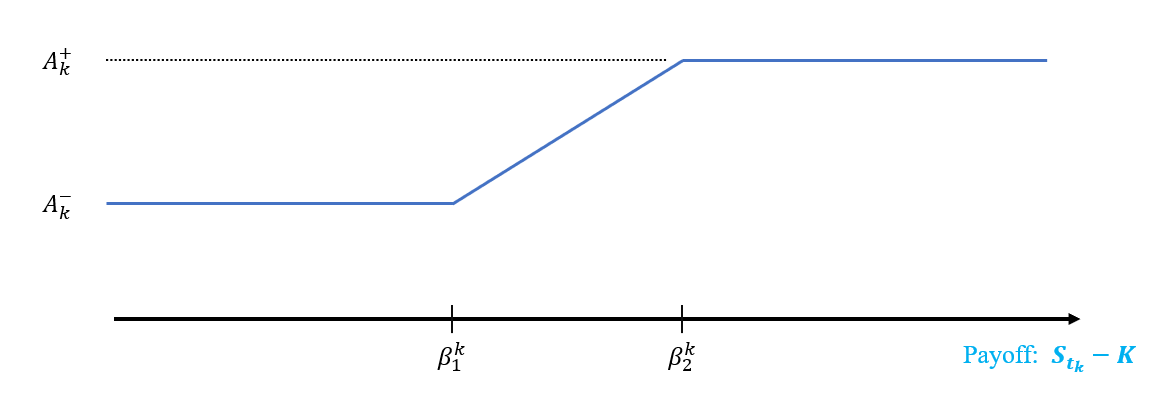
\includegraphics[scale=0.4]{Images/decision_profile.PNG}
    \caption{Optimal consumption profile as a function of the payoff.}
    \label{decision_profile}
\end{figure}


Based on this observation, we aim to find a parametric function that reproduces the consumption profile shown in Figure \ref{decision_profile}, which depends on two thresholds $\beta_1$ and $\beta_2$ (that are assumed to be constant over time in a first step). To achieve this, we define a parametric \q{decision} function

\begin{equation}
        I_k \mapsto f_{k}(I_k; \theta) := f(I_k; \theta) = \mbox{\bf 1}_{\{I_k > \beta_2\}} + \frac{I_k - \beta_1}{\beta_2 - \beta_1}\mbox{\bf 1}_{\{\beta_1 \le I_k \le \beta_2\}}
        \label{strategy_param1}
\end{equation}

\noindent
where $\mbox{\bf 1}$ denotes the indicator function, $\theta = (\beta_1, \beta_2)^\top \in \mathbb{R}^2$ and $I_k = S_{t_k} - K$ is the payoff. Note that the thresholds and therefore the parameterization do not depend on time. The preceding \q{decision} function, once defined, allows to choose an admissible control using the following transformation

\begin{equation}
\label{q_const_loc}
q_k(I_k; \theta) = A_k^{-}(Q_k^\theta) + \Big(A_k^{+}(Q_k^\theta) - A_k^{-}(Q_k^\theta) \Big) \cdot f_{k}(I_k; \theta)
\end{equation}

\noindent
with $Q_0^\theta = 0$ and $Q_k^\theta = \displaystyle \sum_{i = 0}^{k-1} q_i(I_i; \theta)$ for all $1 \le k \le n-1$. Then we aim at solving the parametric optimization problem \eqref{param_prob_init} with the preceding choice of parameterization \eqref{q_const_loc} and with $\Theta = \{(x, y) \in \mathbb{R}^2 ; x < y\}$. To achieve this, we look for values of the thresholds $ \theta  = (\beta_1, \beta_2)$ which maximize the resulting reward function $\mathcal{J}$ (using strategy given by \eqref{strategy_param1}). To implement this approach, we simulate $10^5$ independent realizations of the payoff $I_k = S_{t_k} - K$ and compute the Monte-Carlo price given by strategy \eqref{q_const_loc}. The values of $\beta_1, \beta_2$ used to compute this maximum are the 50 evenly distributed within the interval $[-10, 10]$, for the contract setting of case 2 (as described in section \ref{pricing}).

\begin{comment}
\begin{figure}[!ht]
    \center
    \includegraphics[scale=0.5]{Images/graph_3D_strat.PNG}
    \caption{Swing price with respect to thresholds $\beta_1, \beta_2$.}
    \label{2d_graph_op_strat}
\end{figure}
\end{comment}


The optimal values for $\beta_1$ and $\beta_2$ that lead to the maximum price of $2611.7$ are obtained as $-2.24$ and $-1.02$, respectively. This simple parametric strategy which has no flexibility (the strategy is the same for all exercise dates since thresholds are constants) and does not depend on the cumulative volume (which is obviously essential when deciding which volume to buy at each exercise dates) gives a satisfying price when compared to the more elaborated methods in \cite{BarreraEsteve2006NumericalMF}\footnote{Note the relative error between this price and the best of theirs is roughly $2\%$ and they studied the penalty case whose theoretical price is greater than that of the firm constraints case we study in this paper.}. Following the promising results obtained by this straightforward and simple strategy, we introduce two improvements leading to two different parameterizations.

\begin{itemize}
	\item \textbf{Explicit Payoff-Volume parameterization}: we suppose the optimal consumption behaves like profile \ref{decision_profile} and define a (smooth) parametric function reproducing this profile. The final idea is to use stochastic gradient descent based optimization algorithms to find the best parameters. In this paramterization, we allow the strategy to depend not only on time but also on cumulative consumption. This latter is useful and gives flexibility to our strategy.
	\item \textbf{Neural network parameterization}: this is a variant of the preceding parameterization. Here we replace coefficients which define the first parameterization by the output of a neural network. Once the neural network is trained, we get the parameters and define the same strategy.
\end{itemize}

To illustrate both points of view, we use the settings of case 1 in the following sections.



\subsection{Explicit Payoff-Volume parameterization (\textit{PV strat})}

\indent

We aim to find a parameterization that replicates the target profile in Figure \ref{decision_profile}, and that is also sufficiently regular to allow for optimization using Stochastic Gradient Descent methods. The parameterization needs to be a sufficiently regular function to ensure that the resulting reward function $\mathcal{J}$ is differentiable. To achieve this, we select the logistic function, denoted by $\sigma(x) := \frac{1}{1+e^{-x}}$, which is infinitely differentiable on $\mathbb{R}$ and has a shape close enough to that of the target profile. Additionally, to incorporate flexibility into our exercise strategy, we no longer assume that the parameters are constant over exercise dates. We also need to take into account for the dependence of the strategy on cumulative consumption. Hence, we propose the following parameterization.

    \begin{equation}
        f_{k}(I_k; \theta) = \sigma\big(\langle \theta_k, I_k \rangle  \big)  \hspace{0.8cm} \text{with} \hspace{0.4cm} I_k = \big(S_{t_k} - K, M(Q_k), 1\big)^\top \in \mathbb{R}^3
        \label{strat_qty2}
    \end{equation}
    
\noindent
where for some vector $\theta = (\theta_1, \ldots, \theta_n) \in \Theta = \mathbb{R}^{3n}$, $\theta_k \in \mathbb{R}^3$ ($1 \le k \le n$) is the subvector of $\theta$ made of the $k^{th},(k+1)^{th}, (k+2)^{th}$ components of $\theta$. Thus vector $\theta$ embed all parameters used to define the strategy for all exercise dates. In other words, each $\mathbb{R}^3$-valued component $\theta_k$ represents coefficients that drive the optimal decision of \textit{PV strat} at the corresponding time $t_k$. The function $M$ is chosen as the (normalized) margin or remaining purchasing capacity defined by: $M(Q) := \frac{Q-Q_{\min}}{Q_{\max} - Q_{\min}}$. The importance of this choice is discussed in Remark \ref{rq1} and \ref{rq2}. In case $Q_{\min} = Q_{\max}$, one may use $M(Q) =\frac{Q-Q_{\min}}{Q_{\min}}$. Then the problem to solve is the same as in \eqref{param_prob_init} where the parameters space is $\Theta = \mathbb{R}^{3n}$ and the control $q_k(I_k; \theta)$ in \eqref{q_const_loc} is defined using the strategy \eqref{strat_qty2}.

\begin{remark}[Importance of function $M$]
\label{rq1}
At first glance, the function $M$ may seem to be a simple normalization of the cumulative consumption. However, it should be noted that several other normalizations were tested and did not lead to a good strategy. We tested the following normalizations: $M(Q_k) = Q_k$, $\frac{Q_k - Q_{\min}}{q_{\max} - q_{\min}}$, $\frac{k \cdot q_{\max} - Q_k}{q_{\max} - q_{\min}}$ and $\frac{Q_k - Q^{down}(t_{k+1})}{Q^{up}(t_{k+1}) - Q^{down}(t_{k+1})}$.
\end{remark}

\begin{remark}[Remaining capacity \textit{Versus} Cumulative Consumption]
\label{rq2}
We observed that the remaining purchasing capacity is a more crucial factor than the current cumulative consumption when determining the volume to buy at each exercise date. This contrasts with the neural network approach tested in \cite{BarreraEsteve2006NumericalMF}, which uses the current cumulative consumption. When using $M(Q) = Q$, our algorithm tended to purchase the maximum possible volume at the contract's outset, as long as the payoff was positive. This behavior suggests that the algorithm did not take into account the fact that purchasing capacity diminishes as the contract approaches its expiration, due to global constraints.
\end{remark}

Remarks \ref{rq1} and \ref{rq2} explain the reason for which function $M$ yields desirable results. In addition, this choice has a rational interpretation for the optimal control behavior (see appendix \ref{coeff_explicit_param}).



\subsection{Neural Network parameterization (\textit{NN strat})}
\label{nn_params}

\indent

Our second parameterization is based on neural networks. The goal of a neural network is to approximate some mapping $x \mapsto \Phi^*(x)$ by a parametric one (neural network) $x \mapsto \Phi(x; \theta)$ where $\theta$ is a parameter (or weights) of the neural network that has to be optimized such in order to give a \q{good} approximation. A Neural Network can approximate a wide class of complicated (linear or non-linear) relationships (For more details, see Universal Approximation Theorem \cite{Hornik1989MultilayerFN}) between the inputs and outputs by composing linear functions and non-linear thresholds. More precisely, note that a neural network is made of nodes connected to one another where a column of nodes forms a layer (when there are more than one layer in the neural network architecture, we speak of deep neural network). The outermost (see diagram \ref{nn_representation}) are the input and output layers and all those in between are called the hidden layers. The connection between the input and output layers through hidden layer is made by means of linear functions and activation functions (non-linear ones):


\begin{itemize}
    \item \textbf{Linear functions}: a node in connected to another with an associated weight ($w$) and bias ($b$) so that it will receive a weighted value ($wx+b$) from a node in the previous layer. $\theta = (w,b)$ forms parameters of the neural network.
    \item \textbf{Non-linear functions}: each node contains an activation function that activates the node (so the input can pass through the node) when the input of the node is above a certain threshold.
\end{itemize}



Training a neural network is performed through two steps: \textbf{forward propagation} and \textbf{backward propagation}. The forward propagation leads the predicted output  $\hat{y}$  starting from the input $x$ layer-by-layer. More formally, the forward propagation comes down to the evaluation of the following function:

\begin{equation}
    x \in \mathbb{R}^d \mapsto \Phi(x; \theta) := a_I^{\theta_I} \circ \phi_{q_{I-1}} \circ a_{I-1}^{\theta_{I-1}} \circ \ldots \circ \phi_{q_1} \circ a_1^{\theta_1}(x) \in \mathbb{R}^\ell
    \label{nn_function_rep}
\end{equation}

\noindent
where

\noindent

$\rhd$ $I, q_I, ..., q_1$ are positive integers specifying the depth of the network and the number of nodes for each hidden layer.

$\rhd$ $a_1^{\theta_1}:\mathbb{R}^d \to \mathbb{R}^{q_1},\ldots,a_{I-1}^{\theta_{I-1}}: \mathbb{R}^{q_{I-2}} \to \mathbb{R}^{q_{I-1}}$ and $a_I^{\theta_I}: \mathbb{R}^{q_{I-1}} \to \mathbb{R}^\ell$ are affine functions. As explained above, theses functions are of the form: $a(x) = Wx + b$ where $W$ is a matrix of weights and $b$ is a vector of bias.

$\rhd$ $\text{For} \hspace{0.1cm} j \in \mathbb{N}, \hspace{0.1cm} \phi_j : \mathbb{R}^j \to \mathbb{R}^j$ are the activation functions. In this paper we only use ReLU (Rectified Linear Unit) function i.e, $x \mapsto \max(x, 0)$.


\vspace{0.2cm}

In our case, the neural network is designed/trained to provide a \q{decision} function which maximizes the reward function $\mathcal{J}$. To achieve this, we design a $\mathbb{R}^3$-valued neural network $\Phi(\cdot; \theta)$ (thus $\ell = 3$, see diagram \ref{nn_representation}) of form \eqref{nn_function_rep} and which depends on the time $t_k$, the payoff $S_{t_k} - K$ and the margin $M(Q_k)$ defined as in \eqref{strat_qty2}. Thus $d = 3$ and parameter $\theta$ of the neural network $\Phi(\cdot; \theta)$  lies within

\begin{equation}
\label{param_space}
\Theta = \mathbb{R}^{q_1} \times \mathbb{R}^{3 \times q_1} \times \Big( \prod_{i = 2}^{I-1}  \mathbb{R}^{q_i} \times \mathbb{R}^{q_i \times q_{i-1}}\Big)  \times \mathbb{R}^3 \times \mathbb{R}^{ 3 \times q_{I-1}}.
\end{equation}


\noindent
As for \textit{PV strat}, we define recursively the \q{decision} function by $f_0(I_0; \theta) = \sigma\Big(\langle \Phi\big(t_0, S_{t_0} - K, M(0); \theta\big) , I_0 \rangle\Big) $ and for all $1 \le k \le n-1$


\begin{equation}
\label{nn_parame}
f_k(I_k; \theta) = \sigma\Big(\langle \Phi\big(t_k, S_{t_k} - K, M(Q_k^\theta); \theta\big) , I_k \rangle\Big) \hspace{0.5cm} \text{with} \hspace{0.2cm} Q_k^\theta = \sum_{i = 0}^{k-1} q_i(I_i; \theta)
\end{equation}

\begin{figure}[!ht]
    \center
    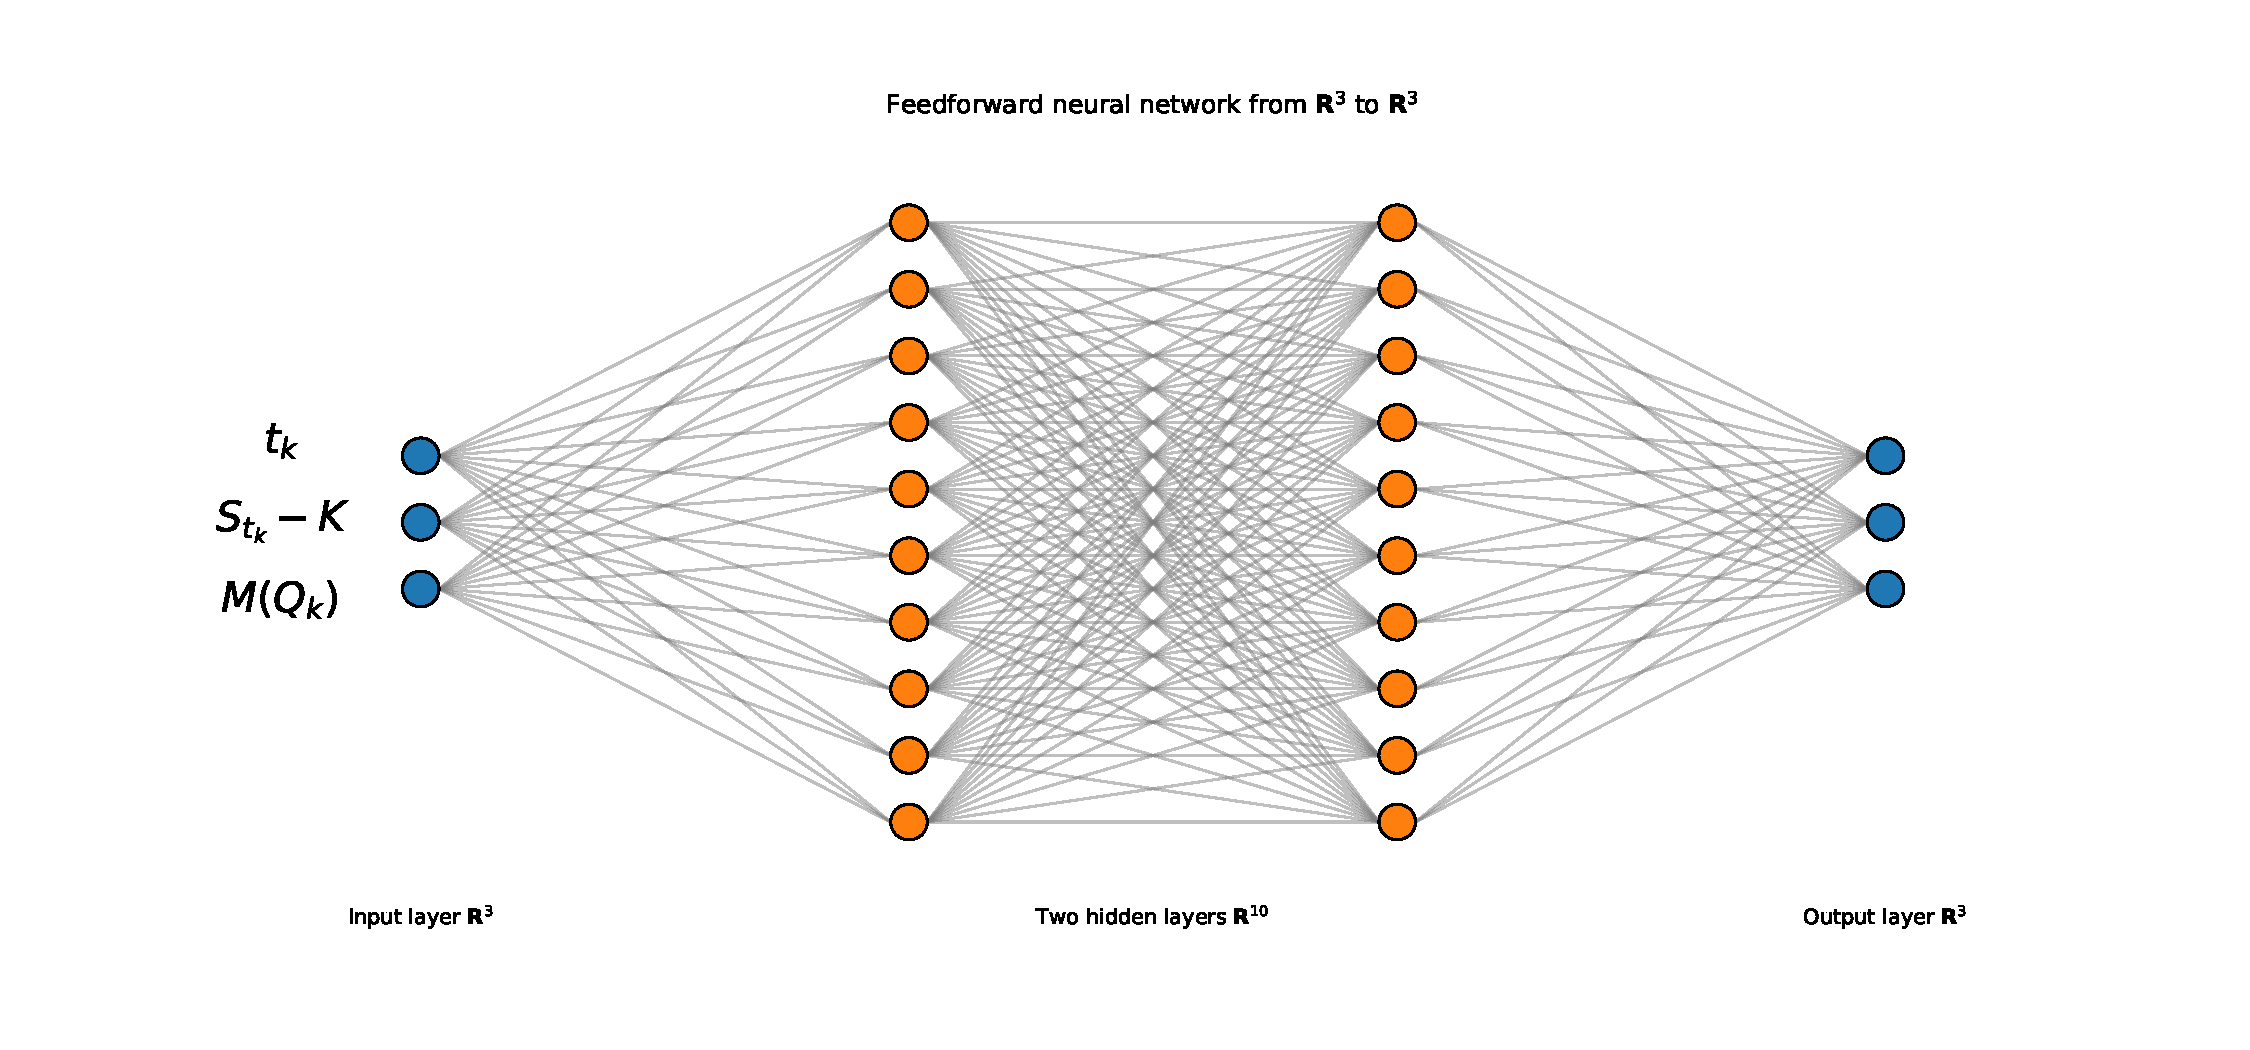
\includegraphics[scale=0.4]{Images/nn_repre.pdf}
    \caption{Illustration of (deep) neural network architecture.}
    \label{nn_representation}
\end{figure}

\noindent
where information $I_k$ is the same as in \eqref{strat_qty2}.Then the parametric optimization problem to solve is the same as defined in equation \eqref{param_prob_init} with the preceding choice of $\Theta$ given by equation \eqref{param_space} and where the control is defined using the strategy \eqref{nn_parame} combined with \eqref{q_const_loc}.

\begin{remark}[\textit{PV strat Versus NN strat}]
Note that in \textit{NN strat}, the parameter $\theta \in \Theta$ (as defined in \eqref{param_space}) replaces all vectors $\theta_k \in \mathbb{R}^3$ in equation \eqref{strat_qty2}, which drives the strategy in \textit{PV strat}. Unlike the latter, in \textit{NN strat}, the same set of parameters defines the strategy for all exercise dates, but the strategy is different according to the exercise date since time is integrated as input. In contrast, the size of the parameter vector in \textit{PV strat} increases linearly with the number of exercise dates. Additionally, in section \ref{transfer_learn}, we will, numerically, demonstrate that even for a high number of exercise dates, a relatively small neural network architecture is still sufficient. This is one of the advantages of \textit{NN strat} over \textit{PV strat}.
\end{remark}

Our neural network parameterization is a more robust one compared to the one performed by Gobet et Al. \cite{BarreraEsteve2006NumericalMF}. Indeed, in their article they had chosen, for the decision function, a non linear $[0,1]$-valued parameterization. Our neural network parameterization is an improvement of theirs in the sense that we first impose a particular parametric shape. Then the parameters that drive the latter shape are chosen as an output of a neural network. This approach not only provides flexibility to the strategy but also helps the algorithm to \q{learn} the optimal control by imposing a specific shape.


All the strategies presented above require training to find the best parameters. To achieve this, we rely on stochastic approximation theory.



\section{Stochastic optimization}
\label{training_part}

\indent

In this section we aim at optimizing a $\mathbb{R}$-valued function $h : y \in \mathbb{R}^q \mapsto \mathbb{E}(H(y, Z))$ with $H$ being a $\mathbb{R}$-valued function defined on $\mathbb{R}^q \times \mathbb{R}^d$ and where $Z$ is a $d-$dimensional random vector. Like a probabilistic extension of the classic Newton-Raphson procedure, stochastic approximation \cite{Kushner2003StochasticAA, Robbins2007ASA}) suggests the following procedure to find zeros of function $h$:

\begin{equation}
    \forall n \in \mathbb{N}, \hspace{0.3cm} y_{n+1} = y_n - \gamma_{n+1} \cdot h(y_n) \hspace{0.4cm}, 0 < \gamma_n \le \gamma_0.
    \label{stoch_algo_iter}
\end{equation}

\noindent
When $h$ is the gradient of another function i.e, $h = \nabla V$, we speak about \textbf{stochastic gradient descent} (SGD) which is an extension of gradient descent (see \cite{Rumelhart1986LearningIR}) to stochastic optimization. Hereafter we consider a SGD setting i.e, $h= \nabla V$. The sequence $(\gamma_n)_{n \in \mathbb{N}}$ is called the algorithm step or learning rate and has to be chosen carefully. In fact if the step is too large, then the procedure \eqref{stoch_algo_iter} can overshoot and completely miss the global optimum of the function $V$. If the step is too small, the procedure may take a long time to converge as it will be taking small steps towards the global minimum. Thus to ensure convergence (which is widely discussed in the literature \cite{EonBottou1998OnlineLA, pmlr-v84-chee18a, Robbins1971ACT}), a classical requirement is the \q{decreasing step} assumption. This means that the step sequence is non-increasing and satisfy the following conditions

\begin{equation}
\label{hyp_DS}
\sum_{n\ge0}^{} \gamma_n = +\infty \hspace{0.3cm} \text{and} \hspace{0.2cm} \sum_{n\ge0}^{} \gamma_n^2 < +\infty.
\end{equation}




From a practical point of view, to implement iteration \eqref{stoch_algo_iter}, one uses mini-batch procedure. That is, rather than computing gradient over a single observation, leading to one iteration in procedure \eqref{stoch_algo_iter}, we use small batches. We divide a sample of size $M$ into $B$ samples of size $L := M / B$. Then we perform $B$ iterations using

\begin{equation}
\label{iter_sgd_MC_mini_batch}
    y_{n+1} = y_n -  \frac{\gamma_{n+1}}{L} \sum_{\ell = 1}^{L} H(y_n, Z_{n+1}^{b, [\ell]}), \hspace{0.3cm} 0 \le n \le N.
\end{equation}

\noindent
where $Z_{n+1}^{b, [\ell]}$ are independent copies of $Z$. This alternative increases update frequency compared to vanilla SGD which allows a more robust convergence, avoiding local minima/maxima. It should be noted that in the SGD framework, $H$ often represents the gradient of a multivariate function, which makes it difficult or impossible to implement the SGD procedure by hand. To address this issue, we use a technique called \q{Adjoint Algorithm Differentiation} (AAD) as described in \cite{Baydin2017AutomaticDI, Paszke2017AutomaticDI}. This technique involves a program that computes a value and automatically computes derivatives of that value by combining the derivatives of several simple arithmetic expressions.




Vanilla SGD can often perform poorly due to various reasons. One of the well-known reasons is its inability to converge or a slow convergence to a local minima/maxima when the objective function has saddle points. A saddle point is a critical point on the surface of the function's graph that is not a local extremum. Saddle points are often found in regions that look like plateaus, as shown in Figure \ref{saddle_pts}.



\begin{figure}[ht]
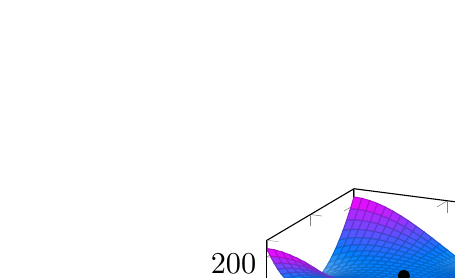
\begin{tikzpicture}
\begin{axis}[
    colormap/cool,
      width=0.4\textwidth,
      height=0.3\textwidth,
]
\addplot3[
    surf,
]
{x^3-3*x*y^2};
\addplot3 [color=black, draw=none, mark=*, mark size=2]table[row sep=crcr] {%
0 0 0\\};
\end{axis}
\end{tikzpicture}
\hskip 80pt
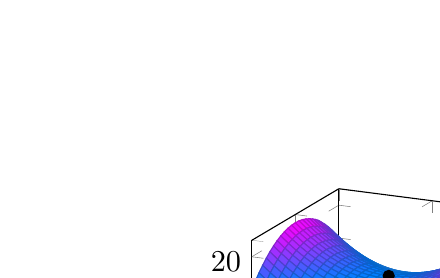
\begin{tikzpicture}
\begin{axis}[
    colormap/cool,
          width=0.4\textwidth,
      height=0.3\textwidth,
]
\addplot3[
    surf,
]
{x^2-y^2};
\addplot3 [color=black, draw=none, mark=*, mark size=2]table[row sep=crcr] {%
0 0 0\\};
\end{axis}
\end{tikzpicture}

\caption{Saddle points illustration. $(x, y) \mapsto x^3 - 3xy^2$ (on left) and $(x, y) \mapsto x^2 - y^2$ (on right). The point $(0,0)$ is a saddle point.}
\label{saddle_pts}
\end{figure}

\noindent
It should be noted that saddle points are notorious in high-dimensional spaces, especially in cases involving deep neural networks, which often have non-convex objective functions (see \cite{Dauphin2014IdentifyingAA, sgdSaddlePoints}). In fact, as the dimensionality of the problem increases, the number of saddle points has been shown to increase exponentially compared to the number of local minima/maxima. For both \textit{PV strat} and \textit{NN strat}, the number of parameters to optimize is high, especially in \textit{NN strat}. Our experiments have shown that vanilla SGD does not perform well in these high-dimensional spaces. Therefore, in this paper, we propose two alternative optimization algorithms, Adaptive Moment Estimation (Adam) and Stochastic Langevin Dynamics (SGLD), and compare their performance.

\subsection{Adaptive Moment Estimation (Adam)}

\indent

Adam \cite{Kingma2015AdamAM} is an efficient stochastic optimization method that only requires first-order gradients with little memory requirement. The method computes individual adaptive learning rates for
different parameters from estimates of first gradient moments. Practically, this is done by means of a preconditioning matrix $P$ (see updating \eqref{langevin_iter}). Adam can be seen at as a combination of RMSprop \footnote{Unpublished optimization algorithm designed for neural networks, first proposed by Geoffrey Hinton in a Coursera course \url{https://www.cs.toronto.edu/~tijmen/csc321/slides/lecture_slides_lec6.pdf}} and Stochastic Gradient Descent with momentum \cite{sgdMoment}. The procedure in Adam updating is the following

\begin{equation}
\label{langevin_iter}
y_{n+1} = y_n - \gamma_{n+1}P_{n+1} \cdot \widehat{\nabla V}(y_n)
\end{equation}

\noindent
where $\widehat{\nabla V}$ is a (scaled) estimation of the gradient (see Algorithm \ref{alg:algorithm1}) computed as a moving average of the estimated gradient in the spirit of momentum technique. $(P_{n})_n$ is a sequence of preconditioning matrix. In Adam updating the latter matrix is a diagonal matrix whose diagonal components depend on the squared (elementwise) of the gradient $g_{n+1}$ estimated after iteration $n$. More precisely, given a gradient $g = \big(g_1, \ldots, g_q \big) \in \mathbb{R}^q$, the square elementwise of this gradient denoted $g \odot g$ is given by

\begin{equation}
\label{sq_elt_grad}
g \odot g = \big(g_1^2, \ldots, g_q^2\big).
\end{equation}

\noindent
In the same spirit, for some matrix $A = \big(a_{i, j} \big)_{1 \le i, j \le q}, B = \big(b_{i, j} \big)_{1 \le i, j \le q}$ where $b_{i, j} \neq 0$ for all $1 \le i, j \le q$ we define elementwise division as follows

\begin{equation}
\label{div_elt_grad}
A \oslash B = \big( c_{i, j} \big)_{1 \le i, j \le q} \hspace{0.6cm} \text{where} \hspace{0.2cm} c_{i, j} = a_{i, j} / b_{i, j}.
\end{equation}


Adam algorithm is described in \ref{alg:algorithm1}.

\newpage


\begin{algorithm}[ht]
  \caption{Adam updating. $\lambda$ is a small correction term to avoid division by zero. $\odot$ denotes elementwise multiplication and $\oslash$ denotes elementwise division defined in \eqref{sq_elt_grad} and \eqref{div_elt_grad}. $Id_q$ represents the $q \times q$ identity matrix.}\label{alg:algorithm1}
  \begin{algorithmic}[1]
    \Require
      \Statex $\rhd$ $\gamma$: Step size
      \Statex $\rhd$ $\mu_1, \mu_2 \in [0, 1)$: Exponential decay rates for the moment estimates
      \Statex $\rhd$ $V(y)$: Stochastic objective function with parameters $y$. Note that $V$ is computed by its Monte-Carlo version using \eqref{iter_sgd_MC_mini_batch}
      \Statex $\rhd$ $y_0$: Initial parameter vector
	\Statex
      \hspace{0.4cm} \Statex $M_0 = 0$ (Initialize $1^{st}$ moment vector)
      \hspace{0.4cm} \Statex $MS_0 = 0$ (Initialize $2^{nd}$ moment vector)
    \Statex
    \While{$y_n$ not converged} 
      \State $g_{n+1} \gets \nabla_y V(y_n)$ \Comment{Compute gradient w.r.t to parameters}
      \State $M_{n+1} \gets \mu_1 \cdot M_n + (1- \mu_1) \cdot g_{n+1}$ \Comment{Update biased first moment estimate}
      \State $MS_{n+1} \gets \mu_2 \cdot MS_n + (1- \mu_2) \cdot g_{n+1} \odot g_{n+1}$ \Comment{Update biased second raw moment estimate}
      \State $\widehat{M}_{n+1} \gets M_{n+1} / (1 - \mu_1^{n+1})$ \Comment{Compute bias-corrected first moment estimate}
      \State $\widehat{MS}_{n+1} \gets MS_{n+1} / (1 - \mu_2^{n+1})$ \Comment{Compute bias-corrected second raw moment estimate}
      \State $P_{n+1} = \diag\Big(Id_q \oslash (\lambda \cdot Id_q + \sqrt{\widehat{MS}_{n+1}}) \Big)$ \Comment{Compute preconditioning matrix}
      \State $y_{n+1} \gets y_n - \gamma \cdot P_{n+1} \cdot \widehat{M}_{n+1}$ \Comment{Update parameters}
    \EndWhile
    
  \end{algorithmic}
\end{algorithm}

Adam uses the squared gradients to scale the learning rate like RMSprop and it takes advantage of momentum by using the moving average (driven by $\mu_1, \mu_2$) of the gradient instead of the gradient itself like SGD with momentum. The scaling of the learning rate by the squared gradient allows to solve gradient magnitude problem. Otherwise, sometimes the gradients may be huge and sometimes small which intricate the choice of a learning rate. The exponential moving average of the gradient allows to \q{de-noise} the estimation of the gradient. Indeed, it is recommended to choose $\mu_1, \mu_2 \approx 1$ so that the contribution of the current estimation of the gradient is small since we give a higher weight to previous data points and lower one to current data points. This allows to smooth subsequent estimation of gradient.


Adam has become the default algorithm for stochastic optimization and especially for neural networks training. Its theoretical convergence had been widely studied in the literature. First, the authors of the algorithm analyzed the convergence in a convex framework with bounded gradient assumption. For non-convex cases, one may refers to \cite{Defossez2020ASC, Zou2018ASC}. 


In this paper, we do not limit our study to Adam updating. We propose to explore other algorithm based on Langevin dynamics and which shares, as Adam, good properties when dealing with saddle points.

\subsection{Preconditioned Stochastic Gradient Langevin Dynamics (PSGLD)}

\indent

Stochastic Gradient Langevin Dynamics (SGLD) has been introduced for bayesian learning \cite{Welling2011BayesianLV} to approximate a posterior distribution given some data. SGLD combines Robbins-Monro type algorithm with Langevin dynamics which injects noise into the parameter updates such
that the trajectory of the parameters converges to the posterior distribution. To be more precise, it has been shown that, under mild conditions, the latter posterior distribution is the unique invariant probability measure of the Langevin Stochastic Differential Equation (SDE):

\begin{equation}
\label{langevin_sde}
dy_t = - \nabla V(y_t) dt + \sqrt{2}dW_t,
\end{equation}

\noindent
where $W$ is a $q$-dimensional Brownian motion. Practically, the posterior distribution is approximated using an Euler discretization of the Langevin SDE

\begin{equation}
\label{langevin_euler}
y_{n+1} = y_n - \gamma \nabla V(y_n)  + \sqrt{2\gamma}Z_{n+1},
\end{equation}

\noindent
where $(Z_{n})_n$ is a sequence of i.i.d. standard $q$-dimensional Gaussian vectors.

From equations \eqref{stoch_algo_iter} (with $h = \nabla V$) and \eqref{langevin_euler}, SGLD appears to be an extension of vanilla SGD by adding an exogenous white noise to the gradient descent. This allows to regularize the problem and escape from traps (see \cite{addgaussnoise}). The use of Langevin dynamics based algorithms for optimization is justified by the fact that recent studies (see \cite{Dalalyan2014TheoreticalGF,Dalalyan2017FurtherAS}) showed that sampling from a distribution which concentrates around the global minimum of $V$ is a similar task as minimizing $V$ via certain optimization algorithms. But, under some conditions, it can be shown (see \cite{Pags2020UnadjustedLA}) that if $(Y_t^y)_{t \ge 0}$ is a $\mathbb{R}^d$-valued random vector solution of the following SDE

\begin{equation}
\label{sde_gen}
dY_t = b(Y_t)dt + \sigma(Y_t) dW_t, \hspace{0.2cm} Y_0 = y
\end{equation}

\noindent
with $W$ a standard $q$-dimensional Brownian motion and a drift term of the form

\begin{equation}
b := -\frac{1}{2} \Big((\sigma \sigma^\top) \nabla V - \Big[\sum_{j = 1}^{d} \partial_{y_j} (\sigma \sigma^\top)_{ij} \Big]_{i =1:d} \Big).
\end{equation}

\noindent
Then, the distribution

\begin{equation}
\nu_V (dy) = C_V e^{-V(y)} \cdot \lambda_d(dy)
\end{equation}

\noindent
is the unique invariant distribution of the SDE \eqref{sde_gen}. In particular if $\sigma = \sqrt{2} \cdot Id_d$ then get the langevin SDE \eqref{langevin_sde}. Which shows that the latter SDE converges to its stationary distribution, namely the Gibbs measure $\propto \exp(-V(y))$ which, in fact, concentrates on the global minimum of $V$. All this motivates the use of Langevin dynamics based algorithms for stochastic optimization (see \cite{ bras2022langevin, PierreLangevin, Jospin_2022}). In this paper, as in \cite{PierreLangevin}, we consider the application of Langevin algorithms in a non-bayesian setting and we will consider the preconditioned version of SGLD which leads to Preconditioned SGLD (PSGLD, see \cite{Li2016PreconditionedSG}). The latter choice is due to the fact that in its standard version, SGLD (without noise) acts like SGD by updating all parameters with the same step size leading to slow mixing when the components of $y$ have different curvature. Given a sequence of preconditioning matrix $(P_n)_n$, the updating procedure \eqref{langevin_euler}, reads in PSGLD setting

\begin{equation}
y_{n+1} = y_n - \gamma_{n+1}P_{n+1} \cdot \nabla V(y_n) + \sigma_{n+1} \sqrt{\gamma_{n+1}} \mathcal{N}(0, P_{n+1})
\end{equation}


\noindent
where $(\sigma_n)_n$ is a constant or non-increasing sequence controlling the amount of injected noise. As in Adam updating the preconditioning matrix sequence $(P_n)_n$ is a diagonal matrix whose components depend on the squared (elementwise) of the gradient estimation. The general procedure is presented in Algorithm \ref{alg:algorithm2}.

\newpage

\begin{algorithm}[ht]
  \caption{PSGLD updating. We take $\sigma_n = \sigma$ and $\gamma_n = \gamma$. $\odot$ and $\oslash$ are defined in \eqref{sq_elt_grad} and \eqref{div_elt_grad}}\label{alg:algorithm2}
  \begin{algorithmic}[1]
    \Require
      \Statex $\rhd$ $\gamma$: Step size
      \Statex $\rhd$ $\mu \in [0, 1)$: Exponential decay rate for the moment squared estimates
      \Statex $\rhd$ $V(y)$: Stochastic objective function with parameters $y$. Note that $V$ is computed by its Monte-Carlo version using \eqref{iter_sgd_MC_mini_batch}
      \Statex $\rhd$ $y_0$: Initial parameter vector
	\Statex
      \hspace{0.4cm} \Statex $MS_0 = 0$ (Initialize $2^{nd}$ moment vector)
    \Statex
    \While{$y_n$ not converged} 
      \State $g_{n+1} \gets \nabla_y V(y_n)$ \Comment{Compute gradient w.r.t to parameters}
      \State $MS_{n+1} = \mu \cdot MS_n + (1 - \mu) \cdot g_{n+1} \odot g_{n+1}$ \Comment{Update biased second raw moment estimate}
      \State $P_{n+1} = \diag\Big(Id_q \oslash (\lambda \cdot Id_q + \sqrt{MS_{n+1}}) \Big)$ \Comment{Compute preconditioning matrix}
      \State $y_{n+1} \gets y_n - \gamma P_{n+1} \cdot g_{n+1} + \sigma \sqrt{\gamma}\cdot \mathcal{N}(0,\,P_{n+1})$ \Comment{Update parameters}
    \EndWhile
    
  \end{algorithmic}
\end{algorithm}

The convergence of Langevin algorithm has been widely studied. One may refers to \cite{langcvg, durmus2018highdimensional} when the sequence $(\sigma_n)_n$ is constant and to \cite{bras:hal-03891234,Pags2020UnadjustedLA} when the sequence is decreasing.


In the next section we implement \textit{PV strat} and \textit{NN strat} with settings of case 1 and optimize them using both Adam and PSGLD presented above.

\subsection{Adam versus PSGLD}
\label{compar_algo}

\indent

We implement \textit{PV strat} and \textit{NN strat} using either Adam or PSGLD optimization algorithm with case 1 setting. For this case the Longstaff-Schwartz method, with canonical polynomial functions of degree 3 provides a price of 65.14 with a 95 \% confidence interval: $[65.08, 65.21]$ and in 4 minutes and 40 second in average. Note that with case 1 (even for case 2) setting, regardless the chosen methods, the resulting Monte-Carlo estimator of the swing price exhibits high variance due to the high variance of the underlying. Thus, in the following table and just for this section, prices are computed by averaging \textit{100 replications} of prices. Each of the 100 prices is obtained using $B = 1$ batch of size $L = M = 2^{14} $ and a learning rate $\gamma = 0.1$. In what follows we denote by $N$ the number of iterations in the stochastic procedure (see \eqref{iter_sgd_MC_mini_batch}), by $\widehat{P_0}$ the (raw) price resulting from \textit{PV strat} or \textit{NN strat}. And $\widehat{P_0}^{BG}$ denotes the price given by forcing the decision function (either \eqref{strat_qty2} for \textit{PV strat} or \eqref{nn_parame} for \textit{NN strat}) to be strictly bang-bang. Results are recorded in Tables \ref{results_explicit_param_comp} and \ref{results_psgld_explicit_param_comp} for \textit{PV strat} and in Tables \ref{results_psgld_explicit_param_comp} and \ref{results_psgld_nn_param_comp} for \textit{NN strat}.



\begin{table}[ht!]
\centering
\begin{tblr}{colspec={c},hlines}
\hline
     $N$ &  $\widehat{P_0}$ &  $\widehat{P_0}^{BG}$ & Time (s) \\
     \hline
     3000 & 65.11 ([65.04, 65.18])& 65.15 ([65.08, 65.22]) & 68.4\\
     1000 & 65.02 ([64.95, 65.08])& 65.18 ([65.12, 65.24]) & 21.3\\
\end{tblr}
\caption{Results for \textit{PV strat} using Adam optimization algorithm. Values in brackets are confidence intervals (95\%). Column \q{time} includes both training and valuation times.}
\label{results_explicit_param_comp}
\end{table}

\newpage


\begin{table}[ht!]
    \centering
\begin{tblr}{colspec={c},hlines}
\hline
     $\sigma$ & $\beta$ & $\widehat{P_0}$ & $\widehat{P_0}^{BG}$ & Time (s) \\
     \hline
     $1 \cdot e^{-6}$ & 0.8  & 65.19 ([65.12, 65.26])& 65.21 ([65.13, 65.28]) & 21.3\\
     $1 \cdot e^{-6}$ & 0.9  & 65.21 ([65.15, 65.28])& 65.23 ([65.17, 65.29]) & 21.3\\
     $1 \cdot e^{-5}$ & 0.9  & 65.22 ([65.16, 65.28])& 65.23 ([65.18, 65.29]) & 21.6\\
\end{tblr}
\caption{Results for \textit{PV strat} using PSGLD optimization algorithm. Values in brackets are confidence intervals (95\%). Column \q{time} includes both training and valuation times. We used $N = 1000$ iterations and $\lambda = 1\cdot e^{-10}$.}
\label{results_psgld_explicit_param_comp}
\end{table}


Tables \ref{results_explicit_param_comp} and \ref{results_psgld_explicit_param_comp} suggest that Adam requires several iterations and, as a result, increases computation time when using a learning rate of 0.1. Whereas with only 1000 iterations, using PSGLD optimization algorithm, leads to a better price. This fact is also observable in  \textit{NN strat} where PSGLD optimization algorithm allows to achieve a better price than Adam.

\begin{table}[ht!]
    \centering
\begin{tblr}{colspec={c},hlines}
\hline
     $N$ &  $\widehat{P_0}$ & $\widehat{P_0}^{BG}$ & Time (s) \\
     \hline
     3000 & 65.22 ([65.16, 65.28])& 65.23 ([65.17, 65.29]) & 150.4\\
     1000 & 65.13 ([65.05, 65.20])& 65.22 ([65.15, 65.29]) & 53.2\\
\end{tblr}
\caption{Results for \textit{NN strat} using Adam optimization algorithm. For the neural network architecture, we used 2 hidden layers ($I = 2$) with 10 units per layer ($q_1 = 10, q_2 = 10$). Values in brackets are confidence intervals (95\%). Columns \q{time} includes the training and the valuation times.}
\label{results_nn_param_1_comp}
\end{table}




\begin{table}[ht!]
    \centering
\begin{tblr}{colspec={c},hlines}
\hline
     $\sigma$ & $\beta$ & $\widehat{P_0}$ & $\widehat{P_0}^{BG}$ & Time (s) \\
     \hline
      $1 \cdot e^{-6}$ & 0.9 & 65.23 ([65.16, 65.30])& 65.21 ([65.14, 65.28]) & 53.4\\
     $1 \cdot e^{-5}$ & 0.9 & 65.23 ([65.14, 65.31])& 65.22 ([65.13, 65.30]) & 52.3\\
     $1 \cdot e^{-6}$ & 0.8 & 65.27 ([65.20, 65.35])& 65.26 ([65.18, 65.33]) & 51.3\\
\end{tblr}
\caption{Results for \textit{NN strat} using PSGLD optimization algorithm. For the neural network architecture, we used 2 hidden layers ($I = 2$) with 10 units per layer ($q_1 = 10, q_2 = 10$). Values in brackets are confidence intervals (95\%). Columns \q{time} includes the training and the valuation times. We used $N = 1000$ iterations and $\lambda = 1\cdot e^{-10}$.}
\label{results_psgld_nn_param_comp}
\end{table}


Tables \ref{results_nn_param_1_comp} and \ref{results_psgld_nn_param_comp} show that prices obtained by \textit{NN strat} are better than that of \textit{PV strat} and, as already mentioned, PSGLD optmization algorithm provides a better exercise strategy. This means that adding some noise in the optimization procedure helps to converge quickly. Following the performance of PSGLD updating, we consider this algorithm in the remainder along with the following configuration: $\sigma = 1 \cdot e^{-6}, \beta = 0.8, \lambda = 1 \cdot e^{-10}$. With the latter setting, one may compute sensitivity of the swing price with respect to the initial forward price (see Figure \ref{deltas_forward}).

\newpage


\begin{figure}[ht]
\centering

\begin{tikzpicture}
\begin{axis}[
	xlabel=Exercise dates,
	ylabel=Delta,
	xmin=0,
	ymin=4,
	grid=both,
	minor grid style={gray!25},
	major grid style={gray!25},
	width=0.5\linewidth,
	height=0.2\paperheight,
	%no marks,
	line width=0.2pt,
	mark size=1.5pt,
	mark options={solid},
	]
\addplot[color=black, mark=*] %
	table[x=time,y=expl,col sep=comma]{datas/greeks/data_30_days.csv};
\addlegendentry{\textit{PV strat}};
\addplot[color=blue, mark=*, style=densely dotted] %
	table[x=time,y=nn,col sep=comma]{datas/greeks/data_30_days.csv};
\addlegendentry{\textit{NN strat}};
\end{axis}
\end{tikzpicture}%
~
\begin{tikzpicture}
\begin{axis}[
	xlabel=Exercise dates,
	ylabel=Delta,
	xmin=0,
	ymin=4,
	grid=both,
	minor grid style={gray!25},
	major grid style={gray!25},
	width=0.5\linewidth,
	height=0.2\paperheight,
	%no marks,
	line width=0.2pt,
	mark size=0.5pt,
	mark options={solid},
	]
\addplot[color=black, mark=*] %
	table[x=time,y=expl,col sep=comma]{datas/greeks/data_365_days.csv};
\addlegendentry{\textit{PV strat}};
\addplot[color=blue, mark=*, style=densely dotted] %
	table[x=time,y=nn,col sep=comma]{datas/greeks/data_365_days.csv};
\addlegendentry{\textit{NN strat}};
\end{axis}
\end{tikzpicture}
\caption{Delta forward for setting of case 1 (left) and case 2 (right) using \textit{PV strat} and \textit{NN strat}.}
\label{deltas_forward}
\end{figure}


Note that for both optimization algorithms (Adam and PSGLD) different other hyperparameters had been tested and results are reported in Appendix \ref{summary_table_algo}.



\subsection{Practitioner's corner: Transfer learning}
\label{transfer_learn}

\indent

As mentioned, in practice, training both parameterizations we proposed in this paper is allowed by AAD. However, the latter can be time consuming especially in the case of a swing contract having several exercise dates and using more than one batch per iteration (see Appendix \ref{summary_table_algo}). For instance, let us consider a swing contract with maturity one year and daily exercise (365 exercise dates). Alongside we use the diffusion  model \eqref{hjm_model} with the setting of case 2. The results are reported in the table below. As observed in \cite{BarreraEsteve2006NumericalMF} the Longstaff-Schwartz method generates numerical instabilities. Moreover, note that we get better prices than optimal quantization method like in \cite{Bardou2009OptimalQF}.


\begin{table}[ht]
    \centering
\begin{tblr}{colspec={c},hlines}
\hline
     &  $\widehat{P_0}$ & $\widehat{P_0}^{BG}$ & $(T_{train}, T_{eval})$ \\
     \hline
     \textbf{\textit{PV strat}}& 2690.10 ([2689.20, 2691.00])& 2692.59 ([2691.68, 2693.49]) & (274.1, 74.7)\\
     \textbf{\textit{NN strat}} & 2693.74 ([2692.83, 2694.64])& 2694.12 ([2693.21, 2695.02]) & (680.9, 398.3) \\
\end{tblr}
\caption{Results for a one-year swing contract. Values in brackets are confidence intervals (95\%). The valuation was performed with a sample of size $1 \cdot e^8$. For the training we used $N = 1000$ iterations. $T_{train}$ denotes the training time and $T_{eval}$ the valuation time.}
\label{one_year_swing_baseline}
\end{table}


From Table \ref{one_year_swing_baseline} one may notice that the computation time is not negligible even if, compared to other methods (like Longstaff-Schwartz) it remains reasonable. To reduce it, we propose a method based on the so called \textbf{transfer learning} (for details see \cite{Pan2010ASO}). Transfer learning refers to a machine learning method where a model developed for a task is reused as the starting point for a model on a second and similar task. This method may accelerates the evaluation of swing contract with several exercise dates. In our case, we perform \q{transfer learning} as follows. For a swing contract with several exercise dates, we first consider an aggregated version. That means that we consider a contract with less exercise dates and where the local constraints are aggregated. For instance for a swing contract over one year with daily exercise and with $q_{\min} = 0, q_{\max} = 6$, we may consider a contract with one exercise per month (the middle of each month) and where for example, for months with 30 days, the local constraints become $q_{\min} = 0 \times 30 = 0, q_{\max} = 30 \times 6 = 180$. Then we run few iterations to optimize the pricing of the aggregated contract. The resulting parameters are used as an initial guess for the actual pricing problem. To extend the parameters obtained in the problem with 12 exercise dates to the problem with 365 exercise dates, we assume that all days within the same month behave the same. Therefore the initial guess parameters for all days within the same month are those obtained in the aggregated problem for this month. It turns out that this allows to reach more quickly a descent optimum.


\begin{table}[ht]
    \centering
\begin{tblr}{colspec={c},hlines}
\hline
      & {$\widehat{P_0}$\\$\widehat{P_0}^{BG}$ } & $T_{agg}$ & $(T_{train}, T_{eval})$ \\
      \hline
     \textbf{\textit{PV strat}}& {2688.73 ([2687.82, 2689.63]) \\2692.81 ([2691.90, 2693.71]) }&  4.8 & (83.2, 76.3)\\
     \textbf{\textit{NN strat}}& {2693.22 ([2692.31, 2694.13]) \\2694.12 ([2693.21, 2695.02]) }& 6.9 & (206.5, 398.1)\\

\end{tblr}
\caption{Results for a one-year swing contract using transfer learning. We used 500 iterations for the aggregated contract and 300 iterations for the actual one-year contract. For the valuation, we used a sample of size $1 \cdot e^8$. $T_{agg}$ denotes the training time for the aggregated contract, $T_{train}$ and $T_{eval}$ denote respectively the training time and the valuation time for the actual contract.}
\label{transfer_learning_one_year_swing}
\end{table}


We can notice from Table \ref{transfer_learning_one_year_swing} that by means of transfer learning the computation time is drastically reduced. With our adaptation of transfer learning, the training time is reduced by a factor of 3 without degrading the accuracy. Besides, always with in mind the aim of reducing the computation time, transfer learning can be used differently. In a few words, by means of transfer learning, when the market data change or when the contracts settings change we do not need to start all over again. To illustrate this point let us consider below three cases: M1, M2, M3, representing some shifts of market/contract settings. Recall that the baseline settings are those consider above (case 2 setting).

\begin{table}[ht]
    \centering
\begin{tblr}{colspec={c},hlines}
\hline
     \textbf{Case M1} & \textbf{Case M2} & \textbf{Case M3}\\
     \hline
     $F_{0, t_k} = 22$ & $\left(Q_{\min}, Q_{\max} \right) = (1400, 2000)$ & $K = 18$\\
\end{tblr}
\caption{Market data move scenarios}
\label{scenario_mkt_move}
\end{table}

\noindent
In Table \ref{scenario_mkt_move} we consider three different market move scenarios described as follows. In the first case we bumped the initial forward curve from 20 to 22. In the second case we change the global constraints from $Q_{\min} = 1300$ and $Q_{\max} = 1900$ to $Q_{\min} = 1400$ and $Q_{\max} = 2000$. In the final case we reduced the strike price from 20 to 18. We could have changed the local constraints but as we already pointed out, swing pricing can always reduce to the case where $q_{\min} = 0, q_{\min} = 1$ (see Appendix \ref{swing decompo}). Now the question is the following: Could our baseline model give accurate prices without training again ? Or could it help us to get accurate prices quickly ? The answers to theses questions are recorded in the following tables.



\begin{table}[ht]
    \centering
\begin{tblr}{colspec={c},hlines}
\hline
     Cases & Re-use & Re-train & $(T_{train}, T_{eval})$ \\
     \hline
     \textbf{Case M1}& {5942.65 ([5941.64, 5943.65]) \\5944.27 ([5943.26, 5945.27]) }& {6005.75 ([6004.70, 6006.79]) \\6008.54 ([6007.50, 6009.58]) } & (85.4, 77.2)\\
     \textbf{Case M2}& {2514.86 ([2513.90, 2515.81]) \\2517.26 ([2516.30, 2518.21]) }& {2516.99 ([2516.04, 2517.93]) \\2518.73 ([2517.78, 2519.67]) } & (85.0, 76.9)\\
     \textbf{Case M3}& {5655.98 ([5655.06, 5656.89]) \\5657.67 ([5656.75, 5658.58]) }& {5744.91 ([5743.95, 5745.86]) \\5747.39 ([5746.43, 5748.34]) } & (85.9, 77.05)\\
\end{tblr}
\caption{Results for \textit{PV strat}. Column \q{Re-use} provides results when the baseline model parameters are reused as is. Column \q{Re-train} gives results when we re-train with only 300 iterations with the baseline model parameters used as starting values. $T_{train}$ denotes the training time and $T_{eval}$ the valuation time. The testing computation time is the same when we re-use the model as when we re-train.}
\label{transfer_learning_mkt_move_strat2}
\end{table}



\begin{table}[ht]
    \centering
\begin{tblr}{colspec={c},hlines}
\hline
     Cases & Re-use & Re-train & $(T_{train}, T_{eval})$ \\
     \hline
     \textbf{Case M1}& {5981.17 ([5980.14, 5982.19]) \\5982.57 ([5981.54, 5983.59]) }& {6011.08 ([6010.03, 6012.12]) \\6011.62 ([6010.57, 6012.66]) } & (203.1, 397.8)\\
     \textbf{Case M2}& {2509.97 ([2509.01, 2510.90]) \\2511.08 ([2510.12, 2512.03]) }& {2516.92 ([2515.96, 2517.87]) \\2517.58 ([2516.62, 2518.53]) } & (203.7, 397.5)\\
     \textbf{Case M3}& {5713.80 ([5712.85, 5714.72]) \\5715.24 ([5714.34, 5716.17]) }& {5749.97 ([5749.01, 5750.92]) \\5750.51 ([5749.55, 5751.46]) } & (203.4, 397.6)\\
\end{tblr}
\caption{Results for \textit{NN strat}. Column \q{Re-use} provides results when the baseline model parameters are reused as is. Column \q{Re-train} gives results when we re-train with only 300 iterations with the baseline model parameters used as starting values. $T_{train}$ denotes the training time and $T_{eval}$ the valuation time. The testing computation time is the same when we re-use the model as when we re-train.}
\label{transfer_learning_mkt_move_strat3}
\end{table}

\newpage

Tables \ref{transfer_learning_mkt_move_strat2} and \ref{transfer_learning_mkt_move_strat3} demonstrate that in the case where global constraints change (M2), using the baseline parameters without additional training gives prices that are comparable to those obtained by training with a few iterations starting from the baseline parameters. Furthermore, it is important to note that increasing the number of iterations beyond 300 (we tested up to 1000 iterations in our experiments) does not lead to better prices than those obtained after 300 iterations (see columns labeled \q{Re-train}). This suggests that reusing the baseline parameters can speed up convergence. This observation remains true regardless of the case (M1, M2, or M3).



\section{Numerical experiments}
\label{sec5}

\indent

We now perform additional simulations to demonstrate the effectiveness of the two parameterizations that we proposed in this paper.


\subsection{Three factor model}

\indent

We first consider a three factor model whose dynamics is given by

\begin{equation}
	\label{3fac_diff}
	\frac{dF_{t, T}}{F_{t_, T}} = \sigma_1 e^{-\alpha_1 (T-t)}dW_t^1 + \sigma_2 e^{-\alpha_2 (T-t)}dW_t^2 + \sigma_3 e^{-\alpha_3 (T-t)}dW_t^3 ,
\end{equation}

\noindent
where for all $1 \le i, j \le 3$, the instantaneous correlation is given by

\begin{equation*}
\langle dW_{\cdot}^i,dW_{\cdot}^j \rangle_t =  \left\{
    \begin{array}{ll}
        dt \hspace{1.4cm} \text{if} \hspace{0.2cm} i = j\\
        \rho_{i, j} \cdot dt \hspace{0.6cm} \text{if} \hspace{0.2cm} i \neq j
    \end{array}
\right.
\end{equation*}

\noindent
In this model, the spot price is given by

\begin{equation*}
S_t = F_{0,t} \cdot \exp\Big(\langle \sigma, X_t \rangle - \frac{1}{2}\lambda_t^2\Big),
\end{equation*}

\noindent
where $\sigma = \big(\sigma_1, \sigma_2, \sigma_3)^\top$, $X_t = \big( X_t^1, X_t^2, X_t^3 \big)^\top $ and for all $1 \le i \le 3$,

\begin{equation*}
X_t^i = \int_{0}^{t} e^{-\alpha_i (t-s)}\, \mathrm{d}W_s^i \hspace{0.3cm} \text{and} \hspace{0.2cm} \lambda_t^2 = \frac{1}{2} \sum_{i = 1}^{3} \frac{\sigma_i^2}{\alpha_i}\big(1-e^{-2\alpha_i t}\big) +  \sum_{i \neq j} \rho_{i, j} \frac{\sigma_i \sigma_j}{\alpha_i + \alpha_j} \Big(1 - e^{-(\alpha_i + \alpha_j)t}  \Big).
\end{equation*}


\noindent
We fix the following configuration $\sigma_i = \sigma = 0.7, \alpha_i = \alpha = 1.5, \rho_{i, j} = \rho \in [-1, 1]$. The swing contract setting corresponds to case 1. We use $N = 1000$ iterations and a learning rate $\gamma = 0.1$. Results are recorded in Tables \ref{three_factor_model_results_strat1} and \ref{three_factor_model_results_strat2}.



\begin{table}[ht]
    \centering
\begin{tblr}{colspec={c},hlines}
\hline
    $\rho$ & $\widehat{P_0}$ & $\widehat{P_0}^{BG}$ \\
    \hline
    0.6 & 172.71 ([172.51, 172.90])& 172.72 ([172.52, 172.92])\\
	0.3 & 147.79 ([147.63, 147.95])& 147.78 ([147.62, 147.95])\\
	-0.2 & 91.02 ([90.92, 91.12])& 91.02 ([90.92, 91.12])\\
\end{tblr}
\caption{Results using \textit{PV strat}. Values in brackets are confidence intervals (95\%). The valuation had been performed with a sample of size $1 \cdot e^8$. For each result, the execution time (training plus testing) is roughly equal to 22s.}
\label{three_factor_model_results_strat1}
\end{table}



\begin{table}[ht]
    \centering
\begin{tblr}{colspec={c},hlines}
\hline
    $\rho$ & $\widehat{P_0}$ & $\widehat{P_0}^{BG}$ \\
    \hline
    0.6 & 173.05 ([172.85, 173.24])& 172.98 ([178.78, 173.17])\\
	0.3 & 147.97 ([147.81, 148.14])& 147.92 ([147.75, 148.08])\\
	-0.2 & 91.18 ([91.08, 91.28])& 91.13 ([91.03, 91.23])\\
\end{tblr}
\caption{Results using \textit{NN strat}. Values in brackets are confidence intervals (95\%). The valuation had been performed with a sample of size $1 \cdot e^8$. For the neural network architecture we used $I = 2$ layers with $q_1 = q_2 = 10$ units. For each result, the execution time (training plus testing) is roughly equal to 45s.}
\label{three_factor_model_results_strat2}
\end{table}



It should be noted that there is a different approach to implement \textit{NN strat}, and taking into account the structure of forward prices. Specifically, in the three-factor framework \eqref{3fac_diff}, the forward price depends on state variables that are components of the $\mathbb{R}^3$-valued random vector $X_t$. In this context, one can include $X_{t_k}$ as an additional input to the neural network described in \eqref{nn_function_rep}, in addition to time $t_k$, payoff $S_{t_k} - K$, and volume normalization $M(Q_k)$. That is, using the above notation, $I_k = \big(t_k, S_{t_k} - K, X_{t_k}, M(Q_k) \big) \in \mathbb{R}^{d+3}$, where $d$ is the dimension of $X_{t_k}$ (in the three-factor model, $d = 3$). This approach can help to capture the correlation structure in a multi-factor framework. The prices resulting from this alternative approach are presented in Table \ref{three_factor_model_results_strat2_state_var}.



\begin{table}[ht]
    \centering
\begin{tblr}{colspec={c},hlines}
\hline
    $\rho$ & $\widehat{P_0}$ & $\widehat{P_0}^{BG}$ \\
    \hline
    0.6 & 172.76 ([172.56, 172.95])& 172.70 ([172.50, 172.89])\\
	0.3 & 147.95 ([147.78, 148.11])& 147.91 ([147.75, 148.07])\\
	-0.2 & 91.11 ([91.01, 91.20])& 91.07 ([90.97, 91.17])\\
\end{tblr}
\caption{Results using \textit{NN strat} including state variables. Values in brackets are confidence intervals (95\%). The valuation had been performed with a sample of size $1 \cdot e^8$. For the neural network architecture we used $I = 2$ layers with $q_1 = q_2 = 10$ units. For each result, the execution time (training plus testing) is roughly equal to 50s.}
\label{three_factor_model_results_strat2_state_var}
\end{table}

It appears that, regardless of whether the model is multi-factor or not, both strategies (\textit{PV strat} and \textit{NN strat}) can determine the optimal volume to purchase at each exercise date, based only on the payoff and the cumulative volume. In the following section, we will evaluate the performance of our strategies on a more complex diffusion model.

\subsection{Multi-curve forward diffusion}

\indent


We finally consider a multi-curve model. At a certain valuation date $t$ we consider $p$ risk factors. Each risk factor $i \in \{1,\ldots,p\}$, denoted by $F_{t, T_i}$, is a forward contract observed at date $t$ and expiring at date $T_i$. It is modeled through an instantaneous volatility function $\sigma_t(T_i)$ with a dynamics given by,

\begin{equation}
\label{BGM}
\frac{dF_{t, T_i}}{F_{t, T_i}} = \sigma_t(T_i) dW_t(T_i)
\end{equation}


\noindent
where $(W_t(T_i))_{t \ge 0}$ is a standard Brownian motion. The instantaneous correlation between Brownian motions are given by

$$\langle dW_{\cdot}(T_i), dW_{\cdot}(T_j) \rangle_t = \rho_{i, j} dt$$

The model \eqref{BGM} implies to diffuse one curve per risk factor; $F_{t, T_i}$ defined by its maturity date $T_i$. Likewise, the spot at a given date generates its own risk factor. Thus if we consider a swing contract on the day-ahead where we can exercise on all working days of a year, then we have about 365 delivery dates. Therefore 365 curves to diffuse. But due to high correlation (at any date, two risk factors are very correlated when maturities are very close), one can see that only a few risk factors really impact the price. In practice forward contracts delivering in the same month are highly correlated. Thus we will consider there are as many factor as months. For example, for a contract on a whole year $p = 12$; therefore 12 (correlated) Brownian motions per exercise date. In this model we consider a valuation date given by $17^{th}$ march 2021 and a swing contract delivering on the period January 2022-December 2022. The swing constraints are: $q_{\min} = 0, q_{\max} = 1, Q_{\min} = 180, Q_{\max} = 270$. For the diffusion model, the correlation matrix is (\textit{in percentage})

\setcounter{MaxMatrixCols}{20}

$$\begin{pmatrix}
100 & 99.62 & 98.61 & 91.12 & 91.12 & 91.12 & 90.24 & 90.24 & 90.24 & 87.2 & 87.2 & 87.2\\
99.62 & 100 & 98.91 & 91.65 & 91.65 & 91.65 & 90.68 & 90.68 & 90.68 & 87.8 & 87.8 & 87.8\\
98.61 & 98.61 & 100 & 93.89 & 93.89 & 93.89 & 92.79 & 92.79 & 92.79 & 89.94 & 89.94 & 89.94\\
91.12 & 91.65 & 93.89 & 100 & 100 & 100 & 99.47 & 99.47 & 99.47 & 97.06 & 97.06 & 97.06\\
91.12 & 91.65 & 93.89 & 100 & 100 & 100 & 99.47 & 99.47 & 99.47 & 97.06 & 97.06 & 97.06\\
91.12 & 91.65 & 93.89 & 100 & 100 & 100 & 99.47 & 99.47 & 99.47 & 97.06 & 97.06 & 97.06\\
90.24 & 90.68 & 92.79 & 99.4 & 99.47 & 99.4 & 100 & 100 & 100 & 97.32 & 97.32 & 97.32\\
90.24 & 90.68 & 92.79 & 99.47 & 99.47 & 99.47 & 100 & 100 & 100 & 97.32 & 97.32 & 97.32\\
90.24 & 90.68 & 92.79 & 99.47 & 99.47 & 99.47 & 100  & 100 & 100 & 97.32 & 97.32 & 97.32\\
87.2 & 87.8 & 89.94 & 97.06 & 97.06 & 97.06 & 97.32 & 97.32 & 97.32 &100 & 100& 100\\
87.2 & 87.8 & 89.94 & 97.06 & 97.06 & 97.06 & 97.32 & 97.32 & 97.32 &100& 100 & 100\\
87.2 & 87.8 & 89.94 & 97.06 & 97.06 & 97.06 & 97.32 & 97.32 & 97.32 & 100 & 100 & 100
\end{pmatrix}$$

\vspace{0.3cm}

\noindent
Volatilities and initial forward prices are assumed to be constant per month. For months in 2022, the square of the instantaneous volatility $\sigma^2_t(T_i)$ is given by Figure \ref{vol_curve_bgm} and the initial forward curve is given by Figure \ref{f0_curve_bgm}.




\begin{figure}[ht!]
\centering
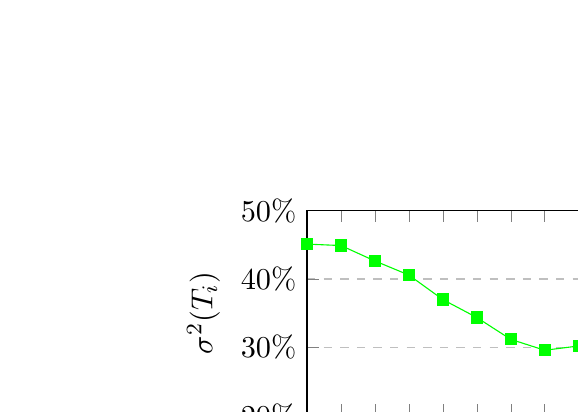
\begin{tikzpicture}
\begin{axis}[
    xlabel={$T_i$},
    ylabel={$\sigma^2(T_i)$},
    xmin=0, xmax=11,
    ymin=20, ymax=50,
    ymajorgrids=true,
    grid style=dashed,
   	width=0.5\linewidth,
	height=0.15\paperheight,
	xticklabels={Jan,Fev,Mar, Apr, May, Jun, Jul, Aug, Sep, Oct, Nov,Dec},xtick={0,...,11},
  x tick label style={rotate=70,anchor=east},
  yticklabel = {\pgfmathprintnumber\tick\%}
]

\addplot[
    color=green,
    mark=square*,
    ]
    coordinates {
    (0,45.09)(1,44.88)(2,42.63)(3,40.57)(4,36.99)(5,34.37)(6,31.18)(7,29.59)(8,30.22)(9,30.60)(10,31.05)(11,30.25)
    };
    
\end{axis}

\end{tikzpicture}
\caption{Square of instantaneous volatility per risk factor observed on 17-March-2021. Values are: $\big(45.09\%,44.88\%,42.63\%,40.57\%,36.99\%,34.37\%,31.18\%,29.59\%,30.22\%,30.6\%,31.05\%,30.25\%\big)$}
\label{vol_curve_bgm}
\end{figure}

\begin{figure}[ht!]
\centering
\begin{tikzpicture}
\begin{axis}[
    xlabel={$T_i$},
    ylabel={$F_{t, T_i}$},
    xmin=0, xmax=11,
    ymin=10, ymax=25,
    ymajorgrids=true,
    grid style=dashed,
   	width=0.5\linewidth,
	height=0.13\paperheight,
	xticklabels={Jan,Fev,Mar, Apr, May, Jun, Jul, Aug, Sep, Oct, Nov,Dec},xtick={0,...,11},
  x tick label style={rotate=70,anchor=east}
]

\addplot[
    color=green,
    mark=square*,
    ]
    coordinates {
    (0,20.07)(1,20.0)(2,19.6)(3,17.4)(4,16.75)(5,16.5)(6,16.56)(7,16.53)(8,16.71)(9,17.31)(10,18.31)(11,18.64)
    };
    
\end{axis}

\end{tikzpicture}
\caption{Forward prices per risk factor observed on 17-March-2021. Prices per risk factor are: $\big(20.07,20,19.6,17.4,16.75,16.5,16.56,16.53,16.71,17.31,18.31,18.64\big)$}
\label{f0_curve_bgm}
\end{figure}


\noindent
Finally, the strike price corresponds to the average of all initial forward prices; which gives 17.865. For this diffusion model, \textit{PV strat} does not perform well. This is probably due to the multi-curve framework which is more complex than a multi factor model. However modifying \textit{NN strat} as in the preceding section by adding, in neural network inputs, Brownian motions $\big(W_{t_k}(T_i)\big)_{1 \le i \le p}$ at each exercise date $t_k$ allows to achieve very good prices. We compare the latter implementation of \textit{NN strat} with a method based on a static replication of swing contracts by means of spread options. The latter method aims at approximating swing options prices by selecting a combination of spread options (\textit{SO}) where the underlying is driven by the same dynamics \eqref{BGM}. The selection is done through a linear programming method. Results are recorded in Table \ref{bgm_strat2_state_var}.



\begin{table}[ht]
    \centering
\begin{tblr}{colspec={c},hlines}
\hline
    $\widehat{P_0}$ & $\widehat{P_0}^{BG}$  & $SO$ \\
    \hline
    708.46 ([705.76, 711.16])& 711.32 ([708.61, 714.03]) & 645.3\\
\end{tblr}
\caption{Results using \textit{NN strat}. Values in brackets are confidence intervals (95\%). The valuation had been performed with a sample of size $5 \times 1\cdot e^{6}$. For the neural network architecture we used $I = 2$ layers with $q_1 = q_2 = 50$ units.}
\label{bgm_strat2_state_var}
\end{table}


\section*{Conclusion}

\indent

We introduced two parametric approaches for pricing swing contracts. The first method involves a direct parameterization of the optimal control based on some heuristics, while the second method improves upon the first by using neural networks. We conducted numerical experiments to compare two optimization algorithms (Adam and PSGLD). Our results demonstrate that using Langevin-based optimization algorithms allows us to achieve better prices with short computation time. We also found that our methods outperform the state-of-the-art methods in terms of accuracy. Additionally, we tested our neural network parameterization in various complex diffusion models and demonstrating its robustness. We can hence conclude that our neural network-based method is well-suited to the pricing swing options.

\section*{Acknowledgments}

The first author is grateful for the financial support provided by Engie Global Markets via CIFRE agreement and would like to thank Asma Meziou and Frederic Muller for throughout insights on swing contracts.

\footnotesize
\appendix

\section{Swing contract decomposition}
\label{swing decompo}

\indent

We aim to prove that any swing contract can be reduced to a normalized contract, namely a swing contract with local constraints $q_{\min} = 0, q_{\max} = 1$. The swing contract price is given by

\begin{equation*}
    P_0 = \esssup_{(q_{\ell})_{0 \le \ell \le n-1} \in \mathcal{A}_{0, 0}^{Q_{\min}, Q_{\max}}} \hspace{0.1cm} \mathbb{E}\left(\sum_{\ell=0}^{n-1} q_{\ell} \times (S_{t_\ell} - K) \right)
\end{equation*}

\noindent
where 

$$\mathcal{A}_{0, 0}^{Q_{\min}, Q_{\max}} = \left\{(q_{\ell})_{0 \le \ell \le n-1}, \hspace{0.1cm} q_{\ell} : (\Omega, \mathcal{F}_{t_\ell}^S, \mathbb{P}) \mapsto [q_{\min}, q_{\max}], \hspace{0.1cm} \sum_{\ell = 0}^{n-1} q_{\ell} \in [Q_{\min}, Q_{\max}] \right\}.$$

\noindent
It follows from the linearity of the expectation that,

\begin{align*}
    P_0 &= q_{\min} \times \mathbb{E}\left(\sum_{\ell=0}^{n-1} (S_{t_\ell} - K) \right) + (q_{\max} - q_{\min}) \times \esssup_{(q_{\ell})_{0 \le \ell \le n-1} \in \mathcal{A}_{0, 0}^{Q_{\min}, Q_{\max}}} \hspace{0.1cm} \mathbb{E}\left(\sum_{\ell=0}^{n-1} \frac{q_{\ell} - q_{\min}}{q_{\max} - q_{\min}} \times (S_{t_\ell} - K) \right).
\end{align*}

\noindent
The first term in the last equality is given by

$$\mathbb{E}\left(\sum_{\ell=0}^{n-1} (S_{t_\ell} - K) \right) = \sum_{\ell=0}^{n-1}\mathbb{E}\left(S_{t_\ell} \right) - n \cdot K$$

\noindent
and can be easily computed using either closed formula (depending on the underlying diffusion model) or Monte-Carlo method. Let us consider the second term. Let $(q_{\ell})_{0 \le \ell \le n-1} \in \mathcal{A}_{0, 0}^{Q_{\min}, Q_{\max}}$ and define $\Tilde{q}_{\ell} = \frac{q_{\ell} - q_{\min}}{q_{\max} - q_{\min}}$. Note that $(\Tilde{q}_{\ell})_{0 \le \ell \le n-1} \in \mathcal{A}_{0, 0}^{\Tilde{Q}_{\min}, \Tilde{Q}_{\max}}$ where


$$\mathcal{A}_{0, 0}^{\Tilde{Q}_{\min}, \Tilde{Q}_{\max}} = \left\{(q_{\ell})_{0 \le \ell \le n-1}, \hspace{0.1cm} q_{\ell} : (\Omega, \mathcal{F}_{t_\ell}, \mathbb{P}) \mapsto [0, 1], \hspace{0.1cm} \sum_{\ell = 0}^{n-1} q_{\ell} \in [\Tilde{Q}_{\min}, \Tilde{Q}_{\max}] \right\}.$$

\noindent
and

$$\Tilde{Q}_{\min} = \frac{(Q_{\min} - n \cdot q_{\min})_{+}}{q_{\max} - q_{\min}} \hspace{0.7cm} \Tilde{Q}_{\max} = \frac{(Q_{\max} - n \cdot q_{\min})_{+}}{q_{\max} - q_{\min}}.$$

\noindent
Thus,

\begin{align*}
    \mathbb{E}\left(\sum_{\ell=0}^{n-1} \frac{q_{\ell} - q_{\min}}{q_{\max} - q_{\min}} \times (S_{t_\ell} - K) \right) &= \mathbb{E}\left(\sum_{\ell=0}^{n-1} \Tilde{q}_{\ell} \times (S_{t_\ell} - K) \right)\\
    &\le \esssup_{(q_{\ell})_{0 \le \ell \le n-1} \in \mathcal{A}_{0, 0}^{\Tilde{Q}_{\min}, \Tilde{Q}_{\max}}}\hspace{0.1cm} \mathbb{E}\left(\sum_{\ell=0}^{n-1} q_{\ell} \times (S_{t_\ell} - K) \right).
\end{align*}

\noindent
Therefore taking the supremum yields,

$$\esssup_{(q_{\ell})_{0 \le \ell \le n-1} \in \mathcal{A}_{0, 0}^{Q_{\min}, Q_{\max}}} \hspace{0.1cm} \mathbb{E}\left(\sum_{\ell=0}^{n-1} \frac{q_{\ell} - q_{\min}}{q_{\max} - q_{\min}} \times (S_{t_\ell} - K) \right) \le \esssup_{(q_{\ell})_{0 \le \ell \le n-1} \in \mathcal{A}_{0, 0}^{\Tilde{Q}_{\min}, \Tilde{Q}_{\max}}} \hspace{0.1cm} \mathbb{E}\left(\sum_{\ell=0}^{n-1} q_{\ell} \times (S_{t_\ell} - K) \right).$$

\noindent
Conversely let $(q_{\ell})_{0 \le \ell \le n-1} \in \mathcal{A}_{0, 0}^{\Tilde{Q}_{\min}, \Tilde{Q}_{\max}}$ and define $\Tilde{q}_{\ell} = q_{\min} + (q_{\max} - q_{\min}) \cdot q_{\ell} \in [q_{\min}, q_{\max}]$. It follows $\displaystyle \sum_{\ell = 0}^{n-1} q_{\ell} \in [Q_{\min}, Q_{\max}]$ so that $\left(\Tilde{q}_{\ell} \right)_{0 \le \ell \le n-1} \in \mathcal{A}_{0, 0}^{Q_{\min}, Q_{\max}}$. Thus,

\begin{align*}
    \mathbb{E}\left(\sum_{\ell=0}^{n-1} q_{\ell} \times (S_{t_\ell} - K) \right) &= \mathbb{E}\left(\sum_{\ell=0}^{n-1} \frac{\Tilde{q}_{\ell} - q_{\min}}{q_{\max} - q_{\min}} \times (S_{t_\ell} - K) \right)\\
    &\le \esssup_{(q_{\ell})_{0 \le \ell \le n-1} \in \mathcal{A}_{0, 0}^{Q_{\min}, Q_{\max}}} \hspace{0.1cm} \mathbb{E}\left(\sum_{\ell=0}^{n-1} \frac{q_{\ell} - q_{\min}}{q_{\max} - q_{\min}} \times (S_{t_\ell} - K) \right).
\end{align*}

\noindent
Taking the supremum, we get,

$$\esssup_{(q_{t_\ell})_{0 \le \ell \le n-1} \in \mathcal{A}_{0, 0}^{\Tilde{Q}_{\min}, \Tilde{Q}_{\max}}} \hspace{0.1cm} \mathbb{E}\left(\sum_{\ell=0}^{n-1} q_{\ell} \times (S_{t_\ell} - K) \right) \le \esssup_{(q_{\ell})_{0 \le \ell \le n-1} \in \mathcal{A}_{0, 0}^{Q_{\min}, Q_{\max}}} \hspace{0.1cm} \mathbb{E}\left(\sum_{\ell=0}^{n-1} \frac{q_{\ell} - q_{\min}}{q_{\max} - q_{\min}} \times (S_{t_\ell} - K) \right).$$

\noindent
Therefore,


\begin{align*}
    P_0 &= q_{\min} \times \mathbb{E}\left(\sum_{\ell=0}^{n-1} (S_{t_\ell} - K) \right) + (q_{\max} - q_{\min}) \times \esssup_{(q_{\ell})_{0 \le \ell \le n-1} \in \mathcal{A}_{0, 0}^{\Tilde{Q}_{\min}, \Tilde{Q}_{\max}}}\hspace{0.1cm} \mathbb{E}\left(\sum_{\ell=0}^{n-1} q_{\ell} \times (S_{t_\ell} - K) \right).
\end{align*}

\section{On the rate of convergence}
\label{sec4}

\indent

This section aims to estimate, at least numerically, the rate of convergence.  We denote by $U_n$ the price obtained after the $n^{th}$ iteration in the training step. We make the assumption that for some constant $C > 0$

$$U_n = U_{\infty} + \frac{C}{n^{\alpha}}$$

\noindent
where $U_{\infty}$ is the limit of the stochastic procedure that we assume to exist. Thus,

$$\log(|U_{2n} - U_{n}|) = K_{\alpha} + \alpha \hspace{0.1cm} \log(\frac{1}{n}), \hspace{0.5cm} \text{where} \hspace{0.1cm} K_{\alpha} = \log(|C(2^{-\alpha} - 1)|).$$

\noindent
Therefore the coefficient $\alpha$ (representing the rate of convergence following the assumption) appears to be the slope in the $\log - \log$ regression of $|U_{2n} - U_{n}|$ against $\frac{1}{n}$.


\begin{figure}[ht!]
  \centering
  \begin{subfigure}[b]{0.45\textwidth}
%%%    \begin{adjustbox}{width=\linewidth} % rescale box
\begin{tikzpicture}{scale = 0.4}
\begin{axis}[
    xmin = 0, xmax = 5,
    ymin = -5, ymax = 5,
    width = 0.9\textwidth,
    height = 0.7\textwidth,
    xtick distance = 1,
    ytick distance = 2,
    grid = both,
    minor tick num = 1,
    major grid style = {lightgray},
    minor grid style = {lightgray!25},
    xlabel = {$\log(n)$},
    ylabel = {$e=\log(|U_{2n} - U_n|)$},
    legend cell align = {left},
    legend pos = south west,
    legend style = {font=\tiny},
    mark size=1.5pt,
]
 
% Plot data
\addplot[
    teal, 
    only marks
] table[x = n, y = e, col sep = comma] {datas/rate_cvg/reg_explicit_30_days.csv};
 
% Linear regression
\addplot[
    thick,
    orange
] table[
    x = n,
    y = {create col/linear regression={y=e}},
    col sep = comma
] {datas/rate_cvg/reg_explicit_30_days.csv};
 
% Add legend
\addlegendentry{Data}
\addlegendentry{
    reg: $ e =
    \pgfmathprintnumber{\pgfplotstableregressiona}
    \cdot log(n)
    \pgfmathprintnumber[print sign]{\pgfplotstableregressionb}$
};
 
\end{axis}
\end{tikzpicture}
\end{subfigure}%
\hfill
\begin{subfigure}[b]{0.45\textwidth}
\begin{tikzpicture}{scale = 0.4}
\begin{axis}[
    xmin = 0, xmax = 5,
    ymin = 0, ymax = 7,
    width = 0.9\textwidth,
    height = 0.7\textwidth,
    xtick distance = 1,
    ytick distance = 2,
    grid = both,
    minor tick num = 1,
    major grid style = {lightgray},
    minor grid style = {lightgray!25},
    xlabel = {$\log(n)$},
    ylabel = {$e=\log(|U_{2n} - U_n|)$},
    legend cell align = {left},
    legend pos = south west,
    legend style = {font=\tiny},
    mark size=1.5pt,
]
 
% Plot data
\addplot[
    teal, 
    only marks
] table[x = n, y = e, col sep = comma] {datas/rate_cvg/reg_explicit_365_days.csv};
 
% Linear regression
\addplot[
    thick,
    orange
] table[
    x = n,
    y = {create col/linear regression={y=e}},
    col sep = comma
] {datas/rate_cvg/reg_explicit_365_days.csv};
 
% Add legend
\addlegendentry{Data}
\addlegendentry{
    reg: $ e =
    \pgfmathprintnumber{\pgfplotstableregressiona}
    \cdot log(n)
    \pgfmathprintnumber[print sign]{\pgfplotstableregressionb}$
};
 
\end{axis}
\end{tikzpicture}
\end{subfigure}
\caption{Numerical Convergence (logarithmic scale) for \textit{PV strat}. Case 1 (left), case 2 (right)}
\label{rate_cvg1}
\end{figure}



\begin{figure}[ht!]
  \centering
  \begin{subfigure}[b]{0.45\textwidth}
%%%    \begin{adjustbox}{width=\linewidth} % rescale box
\begin{tikzpicture}{scale = 0.4}
\begin{axis}[
    xmin = 0, xmax = 5,
    ymin = -4, ymax = 4,
    width = 0.9\textwidth,
    height = 0.7\textwidth,
    xtick distance = 1,
    ytick distance = 2,
    grid = both,
    minor tick num = 1,
    major grid style = {lightgray},
    minor grid style = {lightgray!25},
    xlabel = {$\log(n)$},
    ylabel = {$e=\log(|U_{2n} - U_n|)$},
    legend cell align = {left},
    legend pos = south west,
    legend style = {font=\tiny},
    mark size=1.5pt,
]
 
% Plot data
\addplot[
    teal, 
    only marks
] table[x = n, y = e, col sep = comma] {datas/rate_cvg/reg_nn_30_days.csv};
 
% Linear regression
\addplot[
    thick,
    orange
] table[
    x = n,
    y = {create col/linear regression={y=e}},
    col sep = comma
] {datas/rate_cvg/reg_nn_30_days.csv};
 
% Add legend
\addlegendentry{Data}
\addlegendentry{
    reg: $ e =
    \pgfmathprintnumber{\pgfplotstableregressiona}
    \cdot log(n)
    \pgfmathprintnumber[print sign]{\pgfplotstableregressionb}$
};
 
\end{axis}
\end{tikzpicture}
\end{subfigure}%
\hfill
\begin{subfigure}[b]{0.45\textwidth}
\begin{tikzpicture}{scale = 0.4}
\begin{axis}[
    xmin = 0, xmax = 5,
    ymin = 0, ymax = 7,
    width = 0.9\textwidth,
    height = 0.7\textwidth,
    xtick distance = 1,
    ytick distance = 2,
    grid = both,
    minor tick num = 1,
    major grid style = {lightgray},
    minor grid style = {lightgray!25},
    xlabel = {$\log(n)$},
    ylabel = {$e=\log(|U_{2n} - U_n|)$},
    legend cell align = {left},
    legend pos = south west,
    legend style = {font=\tiny},
    mark size=1.5pt,
]
 
% Plot data
\addplot[
    teal, 
    only marks
] table[x = n, y = e, col sep = comma] {datas/rate_cvg/reg_nn_365_days.csv};
 
% Linear regression
\addplot[
    thick,
    orange
] table[
    x = n,
    y = {create col/linear regression={y=e}},
    col sep = comma
] {datas/rate_cvg/reg_nn_365_days.csv};
 
% Add legend
\addlegendentry{Data}
\addlegendentry{
    reg: $ e =
    \pgfmathprintnumber{\pgfplotstableregressiona}
    \cdot log(n)
    \pgfmathprintnumber[print sign]{\pgfplotstableregressionb}$
};
 
\end{axis}
\end{tikzpicture}
\end{subfigure}
\caption{Numerical Convergence (logarithmic scale) \textit{NN strat}. Case 1 (left), case 2 (right)}
\label{rate_cvg2}
\end{figure}


From figures \ref{rate_cvg1} and \ref{rate_cvg2} it suggests that both parameterizations give a rate of convergence of order $\mathcal{O}(\frac{1}{N})$ (where $N$ is the number of iterations). This convergence rate is much faster than Monte-Carlo, and suggests that our parameterizations are efficient alternatives to Longstaff-Schwartz method for this problem.

\section{Estimator variance and computation time}
\label{add_res}

\indent

In this section we illustrate the high variance phenomenon which may appear when pricing swing option. To this end, we compute 100 realizations of swing contract price with case 1 setting for the three methods: \textit{PV strat}, \textit{NN strat} and Longstaff-Schwartz. The distributions of prices are represented in Figures \ref{var_hist_ep}, \ref{var_hist_nn}, \ref{var_hist_ls}.


\begin{figure}[ht!]
  \centering
  \begin{subfigure}[b]{0.2\textwidth}
    %\begin{adjustbox}{width=\linewidth} % rescale box
    \begin{tikzpicture}
\begin{axis}[
    ybar,
    ymin=1,
    ymax = 100,
    xmin = 62,
    xmax = 68,
    width=1.5\linewidth,
    xtick distance=1,
]
\addplot +[
    hist={
        %bins=1,
        %data min=62,
        %data max=68
    }   
] table[y index = 0]{datas/var_est/var_hist_explicit_param_100000.csv};
\end{axis}
\end{tikzpicture}
\end{subfigure}
\hfill
\begin{subfigure}[b]{0.2\textwidth}
    \begin{tikzpicture}
\begin{axis}[
    ybar,
    ymin=1,
    ymax = 100,
    xmin = 62,
    xmax = 68,
    width=1.5\linewidth,
    xtick distance=1,
]
\addplot +[
    hist={
        %bins=1,
        %data min=62,
        %data max=68
    }   
] table[y index = 0]{datas/var_est/var_hist_explicit_param_1000000.csv};
\end{axis}
\end{tikzpicture}
\end{subfigure}
\hfill
\begin{subfigure}[b]{0.2\textwidth}
    \begin{tikzpicture}
\begin{axis}[
    ybar,
    ymin=1,
    ymax = 100,
    xmin = 62,
    xmax = 68,
    width=1.5\linewidth,
    xtick distance=1,
]
\addplot +[
    hist={
        %bins=1,
        %data min=62,
        %data max=68
    }   
] table[y index = 0]{datas/var_est/var_hist_explicit_param_10000000.csv};
\end{axis}
\end{tikzpicture}
\end{subfigure}
\hfill
\begin{subfigure}[b]{0.2\textwidth}
    \begin{tikzpicture}
\begin{axis}[
    ybar,
    ymin=1,
    ymax = 100,
    xmin = 62,
    xmax = 68,
    width=1.5\linewidth,
    xtick distance=1,
]
\addplot +[
    hist={
        %bins=5,
        %data min=62,
        %data max=68
    }   
] table[y index = 0]{datas/var_est/var_hist_explicit_param_500000000.csv};
\end{axis}
\end{tikzpicture}
\end{subfigure}
\caption{Distribution of swing prices using \textit{PV strat}. From left to right we used successively $10^{5}, 10^{6}, 10^{7}, 5 \times 10^{8}$ simulations.}
\label{var_hist_ep}
\end{figure}



\begin{figure}[ht!]
  \centering
  \begin{subfigure}[b]{0.2\textwidth}
    %\begin{adjustbox}{width=\linewidth} % rescale box
    \begin{tikzpicture}
\begin{axis}[
    ybar,
    ymin=1,
    ymax = 100,
    xmin = 62,
    xmax = 68,
    width=1.5\linewidth,
    xtick distance=1,
]
\addplot +[
    hist={
        %bins=5,
        %data min=62,
        %data max=68
    }   
] table[y index = 0]{datas/var_est/var_hist_nn_param_100000.csv};
\end{axis}
\end{tikzpicture}
\end{subfigure}
\hfill
\begin{subfigure}[b]{0.2\textwidth}
    \begin{tikzpicture}
\begin{axis}[
    ybar,
    ymin=1,
    ymax = 100,
    xmin = 62,
    xmax = 68,
    width=1.5\linewidth,
    xtick distance=1,
]
\addplot +[
    hist={
        %bins=2,
        %data min=62,
        %data max=68
    }   
] table[y index = 0]{datas/var_est/var_hist_nn_param_1000000.csv};
\end{axis}
\end{tikzpicture}
\end{subfigure}
\hfill
\begin{subfigure}[b]{0.2\textwidth}
    \begin{tikzpicture}
\begin{axis}[
    ybar,
    ymin=1,
    ymax = 100,
    xmin = 62,
    xmax = 68,
    width=1.5\linewidth,
    xtick distance=1,
]
\addplot +[
    hist={
        %bins=2,
        %data min=62,
        %data max=68
    }   
] table[y index = 0]{datas/var_est/var_hist_nn_param_10000000.csv};
\end{axis}
\end{tikzpicture}
\end{subfigure}
\hfill
\begin{subfigure}[b]{0.2\textwidth}
    \begin{tikzpicture}
\begin{axis}[
    ybar,
    ymin=1,
    ymax = 100,
    xmin = 62,
    xmax = 68,
    width=1.5\linewidth,
    xtick distance=1,
]
\addplot +[
    hist={
        %bins=1,
        %data min=62,
        %data max=68
    }   
] table[y index = 0]{datas/var_est/var_hist_nn_param_500000000.csv};
\end{axis}
\end{tikzpicture}
\end{subfigure}
\caption{Distribution of swing prices using \textit{NN strat}. From left to right we used successively $10^{5}, 10^{6}, 10^{7}, 5 \times 10^{8}$ simulations.}
\label{var_hist_nn}
\end{figure}


\begin{figure}[ht!]
  %\centering
  \begin{subfigure}[b]{0.2\textwidth}
    %\begin{adjustbox}{width=\linewidth} % rescale box
    \begin{tikzpicture}
\begin{axis}[
    ybar,
    ymin=1,
    ymax = 100,
    xmin = 62,
    xmax = 68,
    width=1.5\linewidth,
    xtick distance=1,
]
\addplot +[
    hist={
        %bins=5,
        %data min=62,
        %data max=68
    }   
] table[y index = 0]{datas/var_est/var_hist_ls_100000.csv};
\end{axis}
\end{tikzpicture}
\end{subfigure}
%\hfill
\hspace*{1.3cm}
\begin{subfigure}[b]{0.2\textwidth}
    \begin{tikzpicture}
\begin{axis}[
    ybar,
    ymin=1,
    ymax = 100,
    xmin = 62,
    xmax = 68,
    width=1.5\linewidth,
    xtick distance=1,
]
\addplot +[
    hist={
        %bins=2,
        %data min=62,
        %data max=68
    }   
] table[y index = 0]{datas/var_est/var_hist_ls_1000000.csv};
\end{axis}
\end{tikzpicture}
\end{subfigure}

\caption{Distribution of swing prices using Longstaff-Schwartz method. From left to right we used successively $10^{5}, 10^{6}$ simulations. Higher number of simulations leads to memory overflow.}
\label{var_hist_ls}
\end{figure}


Figures \ref{var_hist_ep}, \ref{var_hist_nn}, and \ref{var_hist_ls} demonstrate that prices can significantly fluctuate, regardless of the pricing method. Using 1000000 simulations is insufficient to obtain a reliable price estimate. Storage limitations prevent the Longstaff-Schwartz method from exceeding this number of simulations, and this limit is even lower when the number of exercise dates is high. However, our proposed methods allow to increase the number of simulations as needed once the strategy trained. This is possible because we can evaluate our strategies on mini-batches sequentially instead of using the entire test set. For instance, to compute a price with a sample size of $10^8$, we estimate 100 prices over 100 mini-batches, each with a sample size of $10^6$. The final price is then the average of the 100 estimated prices.


Hereafter (see Figure \ref{cpu_time}) we present CPU time for \textit{PV strat} and \textit{NN strat}. We use one batch with size of $2^{14}$ and the same PSGLD setting.


\begin{figure}[ht!]
\centering
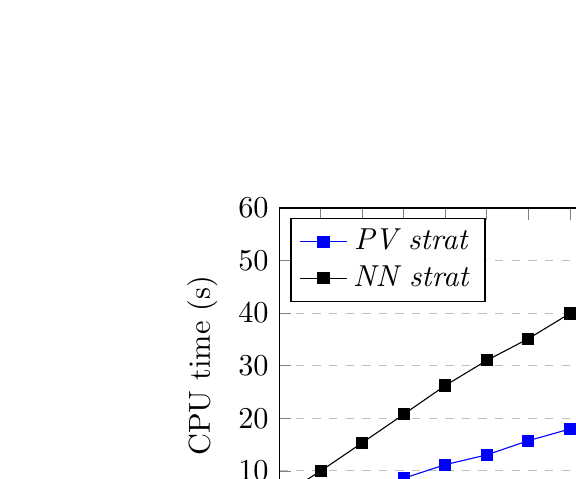
\begin{tikzpicture}
\begin{axis}[
    xlabel={Number of iterations},
    ylabel={CPU time (s)},
    xmin=100, xmax=1000,
    ymin=0, ymax=60,
    xtick={100,200,300,400,500,600,700,800,900,1000},
    ytick={0,10,20,30,40,50,60},
    legend pos=north west,
    ymajorgrids=true,
    grid style=dashed,
   	width=0.5\linewidth,
	height=0.2\paperheight,
]

\addplot[
    color=blue,
    mark=square*,
    ]
    coordinates {
    (100,2.24)(200,4.38)(300,6.61)(400,8.61)(500,11.19)(600,13.05)(700,15.74)(800,17.97)(900,19.69)(1000,20.87)
    };
    %\legend{Strategy 1};
    \addlegendentry{\textit{PV strat}};

\addplot[
    color=black,
    mark=square*,
    ]
    coordinates {
    (100,5.02)(200,9.99)(300,15.35)(400,20.77)(500,26.24)(600,31.02)(700,35.14)(800,39.94)(900,45.11)(1000,51.81)
    };
    %\legend{Strategy 2}
    \addlegendentry{\textit{NN strat}};
    
\end{axis}

\end{tikzpicture}
\caption{CPU time (in seconds) as a function of the number of iterations.}
\label{cpu_time}
\end{figure}


\section{\textit{PV strat} coefficients}
\label{coeff_explicit_param}

\indent

In this appendix we present the coefficients obtained with \textit{PV strat} and either Adam or PSGLD updating. For that purpose, we used $N = 1000$ iterations, a learning rate of 0.1 and the following configurations. For Adam, we use $B = 4$ batches of size $2^{12}$. For the PSGLD updating, we use $\sigma = 1\cdot e^{-6}, \beta = 0.8, \lambda = 1\cdot e^{-10}$ and $B = 1$ batch of size $2^{14}$. In the following graphics, coefficients $a_k, b_k$ represent the coefficients which multiply respectively the payoff $S_{t_k} - K$, the margin of cumulative consumption $M(Q_k)$. The coefficient $c_k$ is the constant (see \eqref{strat_qty2}). For both optimization algorithms, the strategy is estimated with the same sample.


\begin{figure}[ht]
  \centering
  \begin{subfigure}[b]{0.3\textwidth}
    %\begin{adjustbox}{width=\linewidth} % rescale box
    \begin{tikzpicture}
\begin{axis}[
	xlabel=Exercise dates,
	ylabel=$a_k$,
	xmin=0,
	ymin=-8,
	grid=both,
	minor grid style={blue!25},
	major grid style={blue!25},
	every axis legend/.code={\let\addlegendentry\relax},
	width=1.1\linewidth,
	height=0.2\paperheight,
	%no marks,
	line width=1pt,
	mark size=1.5pt,
	mark options={solid},
	]
\addplot[color=black, mark=*]
	table[x=time,y=a_k,col sep=comma]{datas/coeffs_explicit_param/coeff_explcit_param_pSGLD.csv};
\end{axis}
\end{tikzpicture}
\end{subfigure}
\hfill
\begin{subfigure}[b]{0.3\textwidth}
    \begin{tikzpicture}
\begin{axis}[
	xlabel=Exercise dates,
	ylabel=$b_k$,
	xmin=0,
	ymin=-60,
	grid=both,
	minor grid style={blue!25},
	major grid style={blue!25},
	every axis legend/.code={\let\addlegendentry\relax},
	width=1.1\linewidth,
	height=0.2\paperheight,
	%no marks,
	line width=1pt,
	mark size=1.5pt,
	mark options={solid},
	]
\addplot[color=black, mark=*]
	table[x=time,y=b_k,col sep=comma]{datas/coeffs_explicit_param/coeff_explcit_param_pSGLD.csv};
\end{axis}
\end{tikzpicture}
\end{subfigure}
\hfill
\begin{subfigure}[b]{0.3\textwidth}
    \begin{tikzpicture}
\begin{axis}[
	xlabel=Exercise dates,
	ylabel=$c_k$,
	xmin=0,
	ymin=0,
	grid=both,
	minor grid style={blue!25},
	major grid style={blue!25},
	every axis legend/.code={\let\addlegendentry\relax},
	width=1.1\linewidth,
	height=0.2\paperheight,
	%no marks,
	line width=1pt,
	mark size=1.5pt,
	mark options={solid},
	]
\addplot[color=black, mark=*]
	table[x=time,y=c_k,col sep=comma]{datas/coeffs_explicit_param/coeff_explcit_param_pSGLD.csv};
\end{axis}
\end{tikzpicture}
\end{subfigure}
\caption{Coefficients of \textit{PV strat} using PSGLD updating.}
\end{figure}




\begin{figure}[ht]
  \centering
  \begin{subfigure}[b]{0.3\textwidth}
    %\begin{adjustbox}{width=\linewidth} % rescale box
    \begin{tikzpicture}
\begin{axis}[
	xlabel=Exercise dates,
	ylabel=$a_k$,
	xmin=0,
	ymin=-8,
	grid=both,
	minor grid style={blue!25},
	major grid style={blue!25},
	every axis legend/.code={\let\addlegendentry\relax},
	width=1.1\linewidth,
	height=0.2\paperheight,
	%no marks,
	line width=1pt,
	mark size=1.5pt,
	mark options={solid},
	]
\addplot[color=black, mark=*]
	table[x=time,y=a_k,col sep=comma]{datas/coeffs_explicit_param/coeff_explcit_param_Adam.csv};
\end{axis}
\end{tikzpicture}
\end{subfigure}
\hfill
\begin{subfigure}[b]{0.3\textwidth}
    \begin{tikzpicture}
\begin{axis}[
	xlabel=Exercise dates,
	ylabel=$b_k$,
	xmin=0,
	ymin=-80,
	grid=both,
	minor grid style={blue!25},
	major grid style={blue!25},
	every axis legend/.code={\let\addlegendentry\relax},
	width=1.1\linewidth,
	height=0.2\paperheight,
	%no marks,
	line width=1pt,
	mark size=1.5pt,
	mark options={solid},
	]
\addplot[color=black, mark=*]
	table[x=time,y=b_k,col sep=comma]{datas/coeffs_explicit_param/coeff_explcit_param_Adam.csv};
\end{axis}
\end{tikzpicture}
\end{subfigure}
\hfill
\begin{subfigure}[b]{0.3\textwidth}
    \begin{tikzpicture}
\begin{axis}[
	xlabel=Exercise dates,
	ylabel=$c_k$,
	xmin=0,
	ymin=0,
	grid=both,
	minor grid style={blue!25},
	major grid style={blue!25},
	every axis legend/.code={\let\addlegendentry\relax},
	width=1.1\linewidth,
	height=0.2\paperheight,
	%no marks,
	line width=1pt,
	mark size=1.5pt,
	mark options={solid},
	]
\addplot[color=black, mark=*]
	table[x=time,y=c_k,col sep=comma]{datas/coeffs_explicit_param/coeff_explcit_param_Adam.csv};
\end{axis}
\end{tikzpicture}
\end{subfigure}
\caption{Coefficients of \textit{PV strat} using Adam updating.}
\end{figure}


In general, it can be observed that the coefficients estimated using the PSGLD algorithm are smoother across the exercise dates compared to those estimated with the Adam updating method. Additionally, \textit{PV strat} results in interpretable coefficients. Specifically, the coefficient $a_k$ tends to increase globally, with a rapid growth over the last exercise dates. This is because, as we move forward in exercise dates, the minimal global constraint is gradually fulfilled, giving us more flexibility on the control or allowed volumes to purchase. In this particular example, the maximum global constraint is always fulfilled, so towards the last exercise dates, we can decide to buy the minimum possible amount if the payoff is negative and buy the maximum possible amount if the payoff is positive (i.e., the parameterization \eqref{strat_qty2} approaches $0$ or $1$).

On the other hand, the coefficient $b_k$ generally decreases at the beginning of the contract and starts increasing towards zero over the last exercise dates. This indicates that the remaining exercise capacity has less influence on the strategy towards the end of the contract. This is consistent with the claim made earlier, which stated that towards the end of the contract, the optimal strategy depends mainly on the payoff and less on the volume constraints.



\section{Summary tables: Adam versus PSGLD}
\label{summary_table_algo}

\indent

Hereafter are recorded all the results obtained using Adam and PSGLD updatings with different hyperparameters combinations. Prices are computed by averaging 100 replications of prices; each obtained using a sample size of $10^6$. We consider a swing contract with case 1 setting. Results are recorded in tables \ref{results_explicit_param}, \ref{results_nn_param_1}, \ref{results_psgld_explicit_param}, \ref{results_psgld_nn_param}.

\begin{table}[ht]
    \centering
\begin{tblr}{colspec={c},hlines}
\hline
     $L \times B$ & $\gamma$ & $N$ &  $\widehat{P_0}$ &  $\widehat{P_0}^{BG}$ & Time (s) \\
     \hline
     $2^{14} \times 1$ & $0.1$ & 3000 & 65.11 ([65.04, 65.18])& 65.15 ([65.08, 65.22]) & 68.4\\
     $2^{14} \times 1$ & $0.1$ & 1000 & 65.02 ([64.95, 65.08])& 65.18 ([65.12, 65.24]) & 21.3\\
     $2^{12} \times 4$ & $0.1$ & 3000 & 65.14 ([65.08, 65.21])& 65.13 ([65.07, 65.20]) & 261.2\\
     $2^{12} \times 4$ & $0.1$ & 1000 & 65.15 ([65.08, 65.22])& 65.17 ([65.11, 65.24]) & 88.8\\
     $2^{14} \times 1$ & $0.01$ & 3000 & 64.73 ([64.63, 64.79])& 65.05 ([64.98, 65.11]) & 64.4\\
     $2^{14} \times 1$ & $0.01$ & 1000 & 63.91 ([63.83, 63.98])& 64.70 ([64.62, 64.77]) & 22.1\\
     $2^{12} \times 4$ & $0.01$ & 3000 & 65.11 ([65.04, 65.18])& 65.15 ([65.08, 65.22]) & 258.2\\
     $2^{12} \times 4$ & $0.01$ & 1000 & 64.81 ([64.74, 64.88])& 65.03 ([64.98, 65.12]) & 88.3\\
\end{tblr}
\caption{Summary table for \textit{PV strat} using Adam. The values in brackets are confidence intervals (95\%). The column \q{time} includes both training and valuation time.}
\label{results_explicit_param}
\end{table}


\begin{table}[ht]
    \centering
\begin{tblr}{colspec={c},hlines}
\hline
     $L \times B$ & $\gamma$ & $N$ &  $\widehat{P_0}$ &  $\widehat{P_0}^{BG}$ & Time (s) \\
     \hline
     $2^{14} \times 1$ & $0.1$ & 3000 & 65.22 ([65.16, 65.28])& 65.23 ([65.17, 65.29]) & 150.4\\
     $2^{14} \times 1$ & $0.1$ & 1000 & 65.13 ([65.05, 65.20])& 65.22 ([65.15, 65.29]) & 53.2\\
     $2^{12} \times 4$ & $0.1$ & 3000 & 65.26 ([65.21, 65.32])& 65.23 ([65.17, 65.29]) & 603.4\\
     $2^{12} \times 4$ & $0.1$ & 1000 & 65.20 ([65.14, 65.26])& 65.20 ([65.14, 65.26]) & 133.5\\
     $2^{14} \times 1$ & $0.01$ & 3000 & 64.78 ([62.65, 64.90])& 65.06 ([64.98, 65.14]) & 157.1\\
     $2^{14} \times 1$ & $0.01$ & 1000 & 64.81 ([64.74, 64.88])& 65.05 ([64.98, 65.12]) & 55.1\\
     $2^{12} \times 4$ & $0.01$ & 3000 & 65.20 ([65.15, 65.26])& 65.20 ([65.14, 65.26]) & 607.3\\
     $2^{12} \times 4$ & $0.01$ & 1000 & 65.02 ([64.92, 65.11])& 65.17 ([65.09, 65.24]) & 135.4\\
\end{tblr}
\caption{Summary table for \textit{NN strat} using Adam. We used a neural network architecture as follows: 2 hidden layers ($I = 2$) and 10 units per layer ($q_1 = 10, q_2 = 10$). The values in brackets are confidence intervals (95\%). The time includes the training and the valuation time.}
\label{results_nn_param_1}
\end{table}

\newpage


\begin{table}[ht!]
    \centering
\begin{tblr}{colspec={c},hlines}
\hline
     $\sigma$ & $\beta$  &  $\widehat{P_0}$ &  $\widehat{P_0}^{BG}$ & Time (s) \\
     \hline
      $1e^{-5}$ & 0.8  & 65.15 ([65.09, 65.22])& 65.17 ([65.10, 65.23]) & 22.6\\
     $1e^{-5}$ & 0.7  & 65.13 ([65.05, 65.21])& 65.15 ([65.07, 65.22]) & 22.1\\
      $1e^{-5}$ & 0.9 & 65.22 ([65.16, 65.28])& 65.23 ([65.18, 65.29]) & 21.6\\
     $1e^{-6}$ & 0.8  & 65.19 ([65.12, 65.26])& 65.21 ([65.13, 65.28]) & 21.3\\
     $1e^{-6}$ & 0.9  & 65.21 ([65.15, 65.28])& 65.23 ([65.17, 65.29]) & 21.4\\
\end{tblr}
\caption{Summary table for \textit{PV strat} using PSGLD. The values in brackets are confidence intervals (95\%). The column \q{time} includes both training and valuation time. We used a learning rate equal to 0.1, one batch of size $2^{14}$, $\lambda = 1 \cdot e^{-10}$ and 1000 iterations.}
\label{results_psgld_explicit_param}
\end{table}


\begin{table}[ht!]
    \centering
\begin{tblr}{colspec={c},hlines}
\hline
     $\sigma$ & $\beta$ &  $\widehat{P_0}$ &  $\widehat{P_0}^{BG}$ & Time (s) \\
     \hline
      $1e^{-5}$ & 0.8 & 65.18 ([65.12, 65.24])& 65.16 ([65.10, 65.22]) & 53.6\\
      $1e^{-5}$ & 0.7 & 65.22 ([65.15, 65.30])& 65.20 ([65.13, 65.27]) & 52.1\\
      $1e^{-5}$ & 0.9 & 65.23 ([65.14, 65.31])& 65.22 ([65.13, 65.30]) & 52.3\\
     $1e^{-6}$ & 0.8 & 65.27 ([65.20, 65.35])& 65.26 ([65.18, 65.33]) & 51.3\\
     $1e^{-6}$ & 0.9 & 65.23 ([65.16, 65.30])& 65.21 ([65.14, 65.28]) & 53.4\\
\end{tblr}
\caption{Summary table for \textit{NN strat} using PSGLD. We used $I = 2$ layers with $q_1 = q_2 = 10$ units. The values in brackets are confidence intervals (95\%). The column \q{time} includes both training and valuation time. We used a learning rate equal to 0.1, one batch of size $2^{14}$, $\lambda = 1 \cdot e^{-10}$ and 1000 iterations.}
\label{results_psgld_nn_param}
\end{table}

%\nocite{*}
\bibliographystyle{plain}
\bibliography{biblio.bib}

\end{document}
